\cotefile{57}
\scanpage{89}
Donnons-nous une section \deleted{\unsure{de}} $\unsure{\xi}$ de $\underline{\mathrm{Pic}}^{\omega}_{X/S}$ sur $S$, d'où par image inverse une classe de $\mathrm{H}^1(S,\underline{\omega}_{X/S}/\operatorname{Im}f_*(\mathcal{O}_X^*))$, que nous voulons calculer. Pour simplifier, nous \unsure{allons} \unsure{supposer} que $\xi$ provient d'un faisceau inversible $\underline{L}$ sur $X$. Alors on trouve l'image \unsure{de} l'élément de
\[
\mathrm{H}^1(S,\underline{\omega}_{X/S})\simeq\inserted{\operatorname{Ker}}\bigl(\mathrm{H}^1(X,\Omega^1_{X/S})\unsure{\longrightarrow|{-}}\mathrm{H}^0(S,\mathrm{R}^1f_*\unsure{\Omega^1_{X/S}})\bigr)
\]
\unsure{défini} par $\underline{L}$.

\margin{\unsure{1}}
\margin{88}

\scanpage{90}
\margin{89}
\mspage{57}
limit ourselves to the case $g=2$. We are interested in $\mathrm{M}(\Gamma_2(\lambda))$ for $\lambda=1,2$, because we know $\mathrm{S}(\Gamma_2(\lambda))$ explicitly for the same values of $\lambda$ (8). We keep in mind that they are defined as quotient varieties and not as monoidal transforms. We take a point $t_{\unsure{o|0}}$ of $\underline{\mathrm{S}}_1$. Since $t_{\unsure{o|0}}$ is not a fixed point of any element of $\Gamma_1(2)$ different from $\pm1_2$, the analytic local ring $\mathrm{O}$ of $\mathrm{M}(\Gamma_2(2))$ at the image point of $t_{\unsure{o|0}}$ consists of convergent series of the form
\[
\sum_{k=0}^{\infty}\theta_k(t,z)e(kw/2)\ .
\]
The coefficient $\theta_k(t,z)$ is holomorphic in $\mathrm{V}\times\mathbb{C}$ for some $\mathrm{V}$ and $z\longrightarrow\theta_k(t,2z)$ is a theta-function of order $4k$, which is even in the sense it is invariant under $z\longrightarrow-z$. This follows from Theorem 1. Moreover, the ideal $\mathrm{I}$ consists of convergent series which start from $k=1$. Furthermore, there exists a base $(\theta_{\unsure{l|1}}(t_{\unsure{o|0}},z))$ over $\mathbb{C}$ of the vector space of even theta-functions of order four such that each $\theta_{\unsure{l|1}}(t,z)$ is holomorphic in some $\mathrm{V}\times\mathbb{C}$ and such that the correspondence $z\longrightarrow(\theta_{\unsure{l|1}}(t,z))$ gives rise to a complex-analytic embedding of the quotient variety of $\mathrm{T}_1(t)$ by its involution $z\longrightarrow-z$, which is $\mathrm{P}_1(\mathbb{C})$, as a plane curve of order two. Therefore, if we take the monoidal transform of $\mathrm{S}(\Gamma_2(2))$ along its boundary in the neighborhood of the image point of $t_{\unsure{o|0}}$, we get the quotient variety of the monoidal transform of $\mathrm{S}(\Gamma_2(\lambda))$, for any even $\lambda$ at least equal to 3, along its boundary in the neighborhood of the image point of $t_{\unsure{o|0}}$. In the same way, we can conclude that the morphism $\mathrm{M}(\Gamma_2(1))\longrightarrow\mathrm{S}(\Gamma_2(1))$ is a monoidal transformation in the neighborhood of the image point of $t_{\unsure{o|0}}$ provided $t_{\unsure{o|0}}$ is not a fixed point of any element of $\Gamma_1(1)$ different

\scanpage{91}
\uline{NB} Si on a un hom
\[
u:\underline{B}\longrightarrow\underline{\mathrm{Pic}}_{X/S}
\]
avec $B$ un schéma abélien, et si $\underline{\Omega}^1_{X/S}$ \unsure{coh.|est} plat/$S$ en dim 0, alors $u$ se factorise en $B\longrightarrow\underline{\mathrm{Pic}}^\omega_{X/S}$. En particulier, si $\underline{\mathrm{Pic}}^{00}_{X/S}$ existe, alors on a
\[
\underline{\mathrm{Pic}}^{00}_{X/S}\subset\underline{\mathrm{Pic}}^\omega_{X/S}.
\]
Notons que la \uline{donnée} de $u$ équivaut : à \unsure{la} donnée d'un torseur $A$ sous \deleted{\unsure{A}} le schéma dual $B^*$ de $B$, et d'un morphisme
\[
X\longrightarrow A
\]
\margin{sous réserve d'existence de $B^*$ et de \unsure{possibilité} \unsure{en torseurs} (p.ex. si $B/S$ est projectif)}
\[
[\text{d'où}\qquad B\simeq\underline{\mathrm{Pic}}^0_{A/S}\subset\underline{\mathrm{Pic}}_{A/S}\longrightarrow\underline{\mathrm{Pic}}_{X/S}\quad\ldots\ ]
\]
On trouve alors, par fonctorialité, un diagramme
\margin{fonctorialité doit être explicitée avec un peu de soin !}
\diagram{\begin{tikzcd}[column sep=large,row sep=large]
0 \arrow[r,dash] & \underline{\omega}^{\unsure{*|+}}_{X/S} \arrow[r] & M_{X/S} \arrow[r] & \underline{\mathrm{Pic}}^\omega_{X/S} \arrow[r] & 0 \\
0 \arrow[r] & \underline{\omega}_{A/S} \arrow[r]\arrow[u] & M_{A/S} \arrow[r]\arrow[u] & \underline{\mathrm{Pic}}^\omega_{A/S} \arrow[r,dash]\arrow[u] & 0 \\
0 \arrow[r,dash] & \underline{\omega}_{A/S} \arrow[r]\arrow[u,equal] & \deleted{\unsure{E_{B/S}}}\,M^0_{A/S} \arrow[r]\arrow[u] & B \arrow[r]\arrow[u,hook] & 0 \\
& \mathrm{V}(\mathrm{R}^1\unsure{f_{B*}}(\mathcal{O}_B)) \arrow[u,"\simeq"{sloped},draw=none] & & \underline{\mathrm{Pic}}^0_{A/S} \arrow[u,equal] &
\end{tikzcd}}
Ici $\deleted{\unsure{E_{B/S}}}\inserted{M^0_{A/S}}$ est défini comme image inverse de $M_{A/S}$ \inserted{par $B\longrightarrow\underline{\mathrm{Pic}}^\omega_{A/S}$} [ou aussi de $M_{X/S}$ par $B\longrightarrow\underline{\mathrm{Pic}}^\omega_{X/S}$ \inserted{si $\underline{\omega}_{A/S}\simeq\underline{\omega}_{X/S}$}]. Je vou-
\margin{90}

\scanpage{92}
drais l'interpréter comme l'extension \uline{universelle} (de Serre) de $B$ par un fibré vectoriel.

Notons d'abord que le schéma $B^*$ des translations de $\deleted{\unsure{B}}\inserted{A}$ opère \unsure{trivialt} sur l'extension $\deleted{\unsure{E_{A/S}}}\inserted{M^0_{A/S}}$ (car il opère \unsure{trivialt} sur $\underline{\mathrm{Pic}}^0_{A/S}$ et sur $\underline{\omega}_{A/S}$ \deleted{\unsure{\}}}, et $\forall$ hom de $B$ dans $\underline{\omega}_{X/S}$ est trivial). Donc par théorie de descente on voit que $M^0_{A/S}$ est can isom à $M^0_{B^*/S}$, donc c'est un invariant qui ne dépend que du \deleted{\illegible{1}} schéma abélien $B$ sur $S$.

Pour calculer la classe de l'extension obtenue de $\underline{B}$ par $\underline{\omega}_{A/S}$ comme élément de
\[
\mathrm{H}^0\bigl(S,\underbrace{\mathrm{R}^1f_{B*}\deleted{\unsure{*}}(\underline{\omega}_{A/S}\otimes_{\mathcal{O}_S}\mathcal{O}_B)}_{\inserted{\unsure{\mathrm{R}^1f_{B*}(\mathcal{O}_B)^\vee}\otimes\mathrm{R}^1f_{B*}(\mathcal{O}_B)}}\bigr)
\]
on regarde \inserted{par la recette générale} le faisceau inversible canonique sur $P=A\times_S B$, et on écrit l'obstruction à mettre dessus une connexion relative à $B$, i.e. la classe de cohomologie qui lui correspond dans $\mathrm{H}^1(P,\underline{\Omega}^1_{P/B})$ [\unsure{pens. à localiser} sur $S$].
\margin{\diagram{\begin{tikzcd}[column sep=small,row sep=small]
A \arrow[dr,dash,"f_A"'] && B \arrow[dl,dash,"f_B"] \\
& S &
\end{tikzcd}}}
\margin{\diagram{\begin{tikzcd}[column sep=0pt,row sep=small]
A & {}\times_S B \\
B^* \arrow[u,equal] &
\end{tikzcd}}}

Calculons donc la classe de cohomologie de $\underline{L}$ dans $\mathrm{H}^1(A\times_S B,\underline{\Omega}^1_{A\times_S B/S})\deleted{\unsure{\simeq\mathrm{H}}}$, localisé sur $S$.
\margin{91}

\scanpage{93}
\deleted{Cher Monsieur \unsure{Cartan}}
\margin{92}

\scanpage{94}
\[
\begin{aligned}
\underline{\mathrm{H}}^{\unsure{11|1,1}}(A\times_S B)&=\underline{\mathrm{H}}^{\unsure{11|1,1}}(A/S)\oplus\underline{\mathrm{H}}^{\unsure{11|1,1}}(B/S)\\
&\quad+\underline{\mathrm{H}}^{1,0}(A/S)\otimes\underline{\mathrm{H}}^{0,1}(B/S)+\underline{\mathrm{H}}^{0,1}(A/S)\otimes\underline{\mathrm{H}}^{1,0}(B/S)
\end{aligned}
\]
La classe $\xi$ qu'on veut calculer a, pour des raisons de fonctorialité (regarder les inclusions $A\longrightarrow A\times_S B$, $B\unsure{\longrightarrow|{-}}A\times_S B$) des composantes nulles sur les deux premiers facteurs. Il reste à calculer sa classe dans les derniers, on trouve ce qu'on \unsure{pense}\ldots

\figure{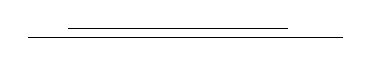
\begin{tikzpicture}\draw (0,0)--(4,0);\draw (.5,.12)--(3.3,.12);\end{tikzpicture}}

\deleted{Connexion \inserted{(absolue)} canonique sur $\underline{M}_{X/S}$}

\deleted{$\underline{W}_{X'_1/S'}\simeq\underline{W}_{X'_2/S'}$ canoniquement ??}

\margin{\diagram{\begin{tikzcd}[column sep=small,row sep=small]
\deleted{X_0} \arrow[r,dash]\arrow[d,dash] & \deleted{\unsure{X'_1}} \arrow[d,dash] & \deleted{\unsure{X''_2}} \arrow[dl,dash] \\
\deleted{S_0} \arrow[r,phantom,"\deleted{\subset}"] & \deleted{\unsure{S'|S''}} &
\end{tikzcd}}
\deleted{dans le voisinage inf. du premier ordre de $S$ avec $\exists$ rétraction de $S$ sur $S_0$}}

\deleted{\uline{Question équivalente}. Si on a un $L_0$ inversible sur $X_0$, muni d'une connexion rel. à $S_0$, alors les \unsure{prolongts} (avec connexions) à $X'$ et à $X''$ se correspondent \unsure{biunivoquement}.}

\margin{$\unsure{W_{X/S}}$}
\margin{$S_0\longleftarrow S$}
\margin{93}

\scanpage{95}
\margin{94}
\mspage{56}
an integer matrix. After this remark, we consider all sequences in $\underline{\mathrm{S}}_g$ of the form $(t,z)\longrightarrow(t_{\unsure{o|0}},z_{\unsure{o|0}})$ and the normal coordinates of $\operatorname{Im}(w)$ tending to $-\infty$ satisfying the condition $y_{12}\geq y_{13},y_{23}$. Then we certainly have $\xi\longrightarrow0$. Moreover, if we take $\theta_{\sigma_{12}}(t,z)$ such that we have $\theta_{\sigma_{12}}(t_{\unsure{o|0}},z_{\unsure{o|0}})\neq0$, the quotient $(\mathrm{H}_\sigma/\mathrm{H}_{\sigma_{12}})(t,z,w)$ is finite along the sequences for every integral, positive, non-degenerate matrix $\sigma$. Among these quotients, we find
\[
(\mathrm{H}_{\sigma_{i3}}/\mathrm{H}_{\sigma_{12}})(t,z,w)=(\theta_{\sigma_{i3}}/\theta_{\sigma_{12}})(t,z)(\xi_{i3}/\xi_{12})(1+\cdots)
\]
for $i=1,2$. Moreover $(\xi_{13}/\xi_{12},\xi_{23}/\xi_{12})$ can approach to any point of the product of two copies of a closed unit disc in $\mathbb{C}$ provided we take the limit $\operatorname{Im}(w)\longrightarrow\infty$ suitably. This implies that the fiber at the image point of $t_{\unsure{o|0}}$ of the monoidal transform of $\mathrm{S}(\Gamma)$ along its boundary is of dimension one more than the fiber of $\mathrm{M}(\Gamma)\longrightarrow\mathrm{S}(\Gamma)$ at the image point of $t_{\unsure{o|0}}$. Therefore $\mathrm{M}(\Gamma)$ is not the monoidal transform of $\mathrm{S}(\Gamma)$ along its boundary. This completes the proof.

We note that the blowing up $\mathrm{M}(\Gamma)\longrightarrow\mathrm{S}(\Gamma)$ can be analyzed along the quasi projective varieties of the form $\Gamma_{\unsure{o|0}}\backslash\underline{\mathrm{S}}_{g_{\unsure{o|0}}}$ for $g_{\unsure{o|0}}=g-1$, contained in the boundary. In fact, it is the partial desingularization of $\mathrm{S}(\Gamma)$ along the image of $\Gamma_{\unsure{o|0}}\backslash\underline{\mathrm{S}}_{g_{\unsure{o|0}}}$, provided $\Gamma$ operates without fixed points on $\underline{\mathrm{S}}_g$ (cf. 10). We also note that most of the groups in the commensurability class of $\operatorname{Sp}(g,\mathbb{Z})$ has ``undesirable'' properties stated for $\Gamma_g(\lambda,2\lambda)$. We shall not try to give a precise form to this statement.

We shall examine $\mathrm{M}(\Gamma_g(\lambda))$ for $\lambda=1,2$. Although a part of the following investigations can be carried out also for $g=3$, we shall

\scanpage{96}
``Critères d'équivalence''
\margin{95}

\scanpage{97}
\fbox{Critères d'équivalence}

$X$ variété projective \deleted{\unsure{géométriquement} \unsure{normale}} \inserted{non sing} de dim $n$

$Y$ section hyperplane \deleted{\unsure{normale}} non sing

$X_m$ m.ième voisinage infinitésimal de $X$

\diagram{\left\{\begin{array}{ll}
\mathrm{Pic}(X)\longrightarrow\mathrm{Pic}(Y)&
\begin{array}{l}
\overbrace{\text{inj si }n\geq3,\ \mathrm{H}^1(Y,\mathcal{O}_Y(\unsure{-m}))=0\text{ pour }m>0;\ \text{surjectif si }n\geq4,\ \mathrm{H}^2(Y,\mathcal{O}_Y(\unsure{-m}))=0\text{ pour }m>0}^{\text{par \unsure{Lef-Grauert}}}\\
\uline{\text{noyau un }p\text{-groupe fini si }n\geq3\ (\text{nul si }Y\text{ général})};\quad\boxed{\text{noyau nul si }n\geq4}
\end{array}\\[1em]
\mathrm{Pic}^{\tau}(X)\longrightarrow\mathrm{Pic}^{\tau}(Y)&
\underbrace{\text{inj. exc. }p\text{ si }n\geq2,\ \text{bij. exc }p\text{ si }n\geq3;\ \text{injectif si }n\geq2\text{ et }Y\ \uline{\text{général}}}_{\text{via }\pi_1,\ \text{\unsure{Lef. Grauert}}}\\[1em]
\mathrm{Pic}^{0}(X)\longrightarrow\mathrm{Pic}^{0}(Y)&
\overbrace{\text{inj exc. }p\text{ si }n\geq2,\ \text{surjectif si }n\geq3,\ \text{bijectif si }n\geq2\text{ et }Y\ \uline{\text{général}}}^{\text{via }\unsure{\pi_1|\pi_2}\quad\text{\unsure{Lef. Grauert}}}
\end{array}\right.}
\margin{$\longleftarrow$ Pic des schémas non \unsure{réduits} \unsure{tels} $X_m$}

\diagram{\begin{array}{lll}
\mathrm{TN}(X)\longrightarrow\mathrm{TN}(Y)&\text{bij exc. }p\text{ si }n\geq3\quad\left[\begin{array}{l}\text{Si }n\geq3,\text{ le noyau est}\\\text{l'image de celui de}\\\mathrm{Pic}^{\tau}(X)\longrightarrow\mathrm{Pic}^{\tau}(Y)\end{array}\right]&\begin{array}{l}\uline{\text{injectif}}\text{ si }Y\ \uline{\text{général}}\\\text{et }n\geq3,\text{ ou}\\\text{si }n\geq4\end{array}\\[1em]
\mathrm{LN}(X)\longrightarrow\mathrm{LN}(Y)&\text{injectif si }n\geq3&\\[1em]
\mathrm{N}(X)\longrightarrow\mathrm{N}(Y)&\begin{array}{l}\text{noyau un }p\text{-groupe fini si }n\geq3\quad\left[\begin{array}{l}\text{contenu exc. }p\\\text{dans l'image}\\\text{du noyau }\deleted{\text{de}}\\\mathrm{Pic}(X)\longrightarrow\mathrm{Pic}(Y),\text{ qui est}\\\text{un }p\text{-groupe fini}\end{array}\right]\end{array}&\begin{array}{l}\text{nul si on a}\\n\geq4\\\uline{\text{ou}}\ Y\ \uline{\text{général}}\end{array}\\[1em]
\underset{m\text{ grand}}{\mathrm{Pic}(X)\longrightarrow\mathrm{Pic}(X_m)}&\text{inj si }n\geq3,\text{ bijectif si }n\geq4&
\end{array}}

\uline{Question} Surjectivité \inserted{(donc bijectivité)} de $\mathrm{Pic}(X)\longrightarrow\mathrm{Pic}(Y)$ \deleted{\unsure{pour}} pour $n\geq4$ sans \uline{conditions cohomologiques}, [\uline{équivalent} à celle de $\deleted{\unsure{T}}\mathrm{N}(X)\longrightarrow\deleted{\unsure{T}}\mathrm{N}(Y)$, ou encore celles de $\mathrm{TN}(X)\longrightarrow\mathrm{TN}(Y)$ et $\mathrm{LN}(X)\longrightarrow\mathrm{LN}(Y)$]. Équivalent à celle de $\mathrm{Pic}(X_m)\longrightarrow\mathrm{Pic}(Y)$ pour $m$ grand. N.B. la surjectivité mod $p^m$ (car. $p>0$) \inserted{[regarder les obstructions successives, \unsure{s'annulent} par $p$\ldots]} \uline{donne pour} $n\geq4$, $\mathrm{Pic}(X)\longrightarrow\mathrm{Pic}(Y)$ \uline{est surjectif exc.} $p$. \deleted{\unsure{Que}} En car. 0, \uline{on peut invoquer la théorie Kählérienne}, qui prouve que \deleted{\illegible{2}} $\mathrm{N}\deleted{\unsure{^{\tau}}}(X)\xrightarrow{\sim}\mathrm{N}(Y)$, d'où $\mathrm{Pic}(X)\longrightarrow\mathrm{Pic}(Y)$.

\margin{Corollaire : $\rho(X)=\rho(Y)$ pour $n\geq4$ [$\rho(X)\leq\rho(Y)$ si $n\geq3$]}
\margin{\deleted{$\unsure{\rho}(X)\leq\rho(Y)$ si $n\geq2$ et $Y$ général}}

\uline{Démonstration} algébrique ???
\margin{96}

\scanpage{99}
\mspage{1}
\uuline{Théorème}\quad $X/k$, $k$ corps \uuline{alg. clos}

$X$ \deleted{\uuline{\unsure{intègre}}}\inserted{\uline{normal} \uline{irréd}} \uuline{projectif}, $X\subset\mathbf{P}^r_k$

\deleted{$\operatorname{prof}X\geq2$ (\unsure{d'où}} \inserted{$\dim X\geq2$} (d'où $\operatorname{prof}X\geq2$)

$G$ groupe algébrique \uuline{affine} \uuline{sans composantes} $\mathrm{G}_m$.
\inserted{(\unsure{p.ex.} un groupe alg. fini).}

$K=\overset{\deleted{\rule{2.7cm}{.3pt}}}{k(t_1,\ldots,t_r)}$, $\overline{K}$ sa clôture algébrique

$Y_{\overline{K}}$ la section hyperplane générique, définie sur $\overline{K}$.

Alors
\[
\mathrm{H}^1(X,G)\longrightarrow\mathrm{H}^1(Y_{\overline{K}},G)\qquad\uuline{\text{est injectif}}
\]
La structure des groupes algébriques \unsure{comm.} nous ramène aux cas simples $\mathrm{G}_a$, \deleted{$\unsure{\mathrm{G}_m}$}, groupe fini simple, \inserted{$\alpha_p$}, $\mu_p$.

Donc on est ramené à prouver

\uline{Corollaire 1}\quad $\mathrm{H}^1(X,\underline{\mathcal{O}}_X)\longrightarrow\mathrm{H}^1(Y_{\overline{K}},\underline{\mathcal{O}}_{Y_{\overline{K}}})$ est injectif

\margin{N.B. \unsure{Généraliser} au cas d'un morphisme dominant $X\longrightarrow\mathbf{P}^r$}

\deleted{\uline{Corollaire 2}\quad $\mathrm{Pic}(X)\longrightarrow\mathrm{Pic}(Y_{\overline{K}})$ est injectif}

\uline{Corollaire 2}\quad $\pi_1(Y_{\overline{K}})\longrightarrow\pi_1(X)$ est surjectif\quad [C'est \uuline{Bertini}]

\uline{Corollaire 3}\quad $\mathrm{H}^1(X,\alpha_p)\unsure{{-}|\longrightarrow}\mathrm{H}^1(\unsure{X|Y}_{\overline{K}},\alpha_p)$ injectif

\uline{Corollaire 4}\quad $\mathrm{H}^1(X,\mu_p)\unsure{{-}|\longrightarrow}\mathrm{H}^1(Y_{\overline{K}},\mu_p)$ injectif.

On part du corollaire 2, connu grâce à Bertini; \uline{ou} Lefschetz-Grauert [\unsure{utilise} \unsure{déjà que} $\operatorname{prof}X\geq2$]. On en déduit
\[
\mathrm{H}^1(X,\underline{\mathcal{O}}_X)^F\Rightarrow\mathrm{H}^1(X,\mathbf{Z}/p\mathbf{Z})\longrightarrow\mathrm{H}^1(Y_{\overline{K}},\underline{\mathcal{O}}_{Y_{\overline{K}}})^F
\]
est injectif, on est donc ramené pour le cor. 1 de prouver que
\[
\mathrm{H}^1(X,\underline{\mathcal{O}}_X)^{1-F}\unsure{{-}|\longrightarrow}\mathrm{H}^1(Y_{\overline{K}},\underline{\mathcal{O}}_{Y_{\overline{K}}})^{1-F}
\]
est injectif [N.B. en tous cas le noyau est stable sous $F$\ldots] i.e. au corollaire 3. Donc on est ramené \inserted{\uline{En car.} $p>0$} \deleted{\illegible{1}} au cas des cor. 3. et 4. En car $p=0$,
\margin{98}

\scanpage{100}
\deleted{\unsure{provenant} de $\mathrm{H}^1(X,G)$, \unsure{prouver} \unsure{par} \unsure{un} \inserted{\unsure{petit}} \unsure{argument} \unsure{positif}}

On utilisera un argument de spécialisation.

\unsure{On en} \deleted{\unsure{partant de}} \inserted{\unsure{suivant}} Cartier, de la suite exacte
\[
0\unsure{{-}|\longrightarrow}\underline{\mathcal{O}}_X\xrightarrow{F}\underline{\mathcal{O}}_X\longrightarrow\underline{\mathcal{O}}_X/\underline{\mathcal{O}}_X^p\unsure{{-}|\longrightarrow}0
\]
\[
1\unsure{{-}|\longrightarrow}\underline{\mathcal{O}}_X^*\xrightarrow{F}\underline{\mathcal{O}}_X^*\unsure{{-}|\longrightarrow}\underline{\mathcal{O}}_X^*/\underline{\mathcal{O}}_X^{*p}\longrightarrow1
\]
\margin{($X$ intègre !)}
\deleted{\unsure{on tire}} on tire
\[
\mathrm{H}^1(X,\alpha_p)=\mathrm{H}^1(X,\underline{\mathcal{O}}_X)^{1-F}\simeq\mathrm{H}^0(X,\underline{\mathcal{O}}_X/\underline{\mathcal{O}}_X^p)\xrightarrow{df}\mathrm{H}^0(X,\underline{\widetilde{\Omega}}^1_X)
\]
\[
\mathrm{H}^1(X,\mu_p)=\mathrm{H}^1(X,\underline{\mathcal{O}}_X)^{1-F}\simeq\mathrm{H}^0(X,\underline{\mathcal{O}}_X/\underline{\mathcal{O}}_X^*)\xrightarrow{\frac{df}{f}}\mathrm{H}^0(X,\underline{\widetilde{\Omega}}^1_X)
\]
et si $X$ est \uline{normal} les deux flèches écrites sont injectives [\deleted{\unsure{leurs}}\inserted{en tous cas,} les noyaux s'identifient, soit aux \uline{diviseurs additifs} sur $X$ annulés par $F$, soit aux diviseurs multiplicatifs annulés par $F$].

Donc on est ramené au

\uline{Lemme}\quad $\mathrm{H}^0(X,\widetilde{\Omega}^1_{X/k})\longrightarrow\mathrm{H}^0(Y_{\overline{K}},\widetilde{\Omega}^1_{Y_{\overline{K}}/\overline{K}})$ est injectif.

La vérification est presque triviale\ldots

\uline{Corollaire}\quad $\underline{\mathrm{Pic}}^\tau_{X_{\overline{K}}/\overline{K}}\longrightarrow\underline{\mathrm{Pic}}^\tau_{\unsure{X|Y}_{\overline{K}}/\overline{K}}$ a un noyau qui est un \uline{$p$-groupe fini unipotent}, [le fait qu'il est complet résulte déjà de $\operatorname{prof}X\geq2$, grâce au \deleted{Bertini} Lefschetz-Grauert-Bertini], ``sans partie fixe''. Si $X$ est normal (pas néc. de $\dim\geq2$), \inserted{$\underline{\mathrm{Pic}}^{\unsure{0|\tau}}_{X/k}$ est propre sur $k$.}
\margin{purement infinitésimal}

Le ``sans partie fixe'' provient de la normalité; elle explique que l'on a une \uline{immersion} \uline{finie} $\underline{\mathrm{Pic}}^\tau_{X/k}\longrightarrow\prod_i\underline{\mathrm{Pic}}_{Y_i/k}$, les $Y_i$ des sections hyperplanes \unsure{rendues} normales. Donc pour prouver
\margin{99}

\scanpage{101}
que $\underline{\operatorname{Pic}}^\tau_{X/k}$ est propre, on se ramène à le prouver pour une \uline{courbe} normale, et c'est connu. Alors un sous-gr. \unsure{unip.} est néc. fini, ce qui achève de prouver l'assertion\ldots.

\figure{\begin{tikzpicture}\draw (0,0)--(.6,0);\end{tikzpicture}}

\uline{Démonstration directe et indépendante de la coh. du fait que si $X$ est \inserted{géom\textsuperscript{t}} normal et projectif$/k$}, \deleted{\unsure{alors}} $\underline{\operatorname{Pic}}^0_{X/k}$ est propre.

On utilise le théorème de structure des groupes algébriques commutatifs, on est ramené à prouver que toute application $\operatorname{Spec}(k[t,t^{-1}])\longrightarrow\underline{\operatorname{Pic}}^0_{X/k}$ est constante, \deleted{et il suffit [$k$ clos alg. \unsure{clos}] de prouver que l'application \inserted{ens.} sous-jacente est triviale \unsure{des points du} \unsure{corps}.}

\margin{\unsure{Prendre} un \unsure{fermé} $Y$ de codim $\geq2$ \deleted{dont} \unsure{tel que} $U:X-Y$ \unsure{soit régulier}.}

\uline{Lemme} Supposons $X$ \unsure{noethérien} \unsure{localt} normal. Alors \deleted{\unsure{pour tout}}
\[
 \operatorname{Pic}(X)\longrightarrow\operatorname{Pic}X[t,t^{-1}]
\]
est \deleted{bijectif} \uline{surjectif}.

\margin{Certainement inutile, en procédant de façon \unsure{annuelle|annulée}.}

\deleted{C'est injectif, car $X[t]$ a une section sur $X$ (section unité).} Soit donc $\underline L$ faisceau inversible sur $X'=X[t,t^{-1}]$, \deleted{soit $U\longrightarrow X$, \unsure{ouvert de} \unsure{la} \unsure{régularité} de $X$} \inserted{\unsure{Prenons} $U'=X'(U)$} $\underline L\mid U'\deleted{\unsure{[t]}}$ provient d'un faisceau inversible $\underline L_0$ sur $U$, qui est défini à l'aide d'un diviseur $D_0$ sur $U$. Son \unsure{adhérence} $D_1=\overline{D}_0$ est tq que son image inverse sur $X'\deleted{\unsure{[t]}}$ \deleted{\unsure{est}} soit loc. principale. Par raison de platitude, il en est de $=$ de $D_1$, d'où facilement la conclusion.
\margin{100}

\scanpage{102}
[ N.B. \uline{Lemme} $X$ préschéma, $U$ ouvert rétro-compact, $f:X'\mathbin{-}X$ morphisme \uline{fid plat} et \uline{qu cpt}, $U'=f^{-1}(\unsure{X'|U})$, on suppose $\boxed{i'_*(\mathcal O_{U'})\simeq\mathcal O_{X'}}$. (ce qui est équivalent à la formule $\boxed{i_*(\mathcal O_U)\simeq\mathcal O_X}$).

\margin{\diagram{\begin{tikzcd}[column sep=small,row sep=small]
 \underline E' & {}\\
 X'\arrow[d,"f"'] & U'\arrow[l,hook',"i'"']\arrow[d,"g"]\\
 X & U\arrow[l,hook',"i"']\\
 {} & \underline F
 \end{tikzcd}}}

Soit $P(X)$ l'ens des classes, à isom près, de faisceaux loc. libres de type fini sur $X$, définissons de $=$ $P(X')$, $P(U)$, $P(U')$. Alors le diagramme
\diagram{\begin{tikzcd}
 P(X)\arrow[r,dash]\arrow[d] & P(X')\arrow[d]\\
 P(U)\arrow[r,dash] & P(U')
\end{tikzcd}}
\unsure{est} \uline{cartésien} \deleted{\unsure{cartésien}}. En particulier, le diagramme
\diagram{\begin{tikzcd}
 \operatorname{Pic}(X)\arrow[r]\arrow[d] & \operatorname{Pic}(X')\arrow[d]\\
 \operatorname{Pic}(U)\arrow[r] & \operatorname{Pic}(U')
\end{tikzcd}}
est \uline{cartésien}.

\margin{N.B. Inutile de se borner à des faisceaux loc. libres. On peut \unsure{admettre} \unsure{tous} les faisceaux $\underline E$ tels que $\operatorname{prof}E_x\geq2$ pour $x\in X-U$, et $\underline E'$ en \unsure{conséquence}\ldots\ [en loc. noeth].}

En effet, \deleted{\unsure{si}} le foncteur $\underline E\longmapsto i^*(\underline E)$ des $\underline E$ loc libres sur $X$ en les \unsure{faisc} loc libres sur $U$ est \uline{pleinement fidèle}, donc $P(X)\mathbin{-}P(U)$ est injectif, [et de $=$ $P(X')\longrightarrow P(U')$ l'est] donc
\[
 P(X)\mathbin{-}P(U)\mathop{\times}_{P(U')}P(X')
\]
est injectif. \deleted{\unsure{Soient d'abord}} \inserted{Prouvons la} surjectivité. Soient $\underline F$ loc. libre sur $U$, $\underline E'$ loc. libre sur $X'$, tels que $i'^*(\underline E')\simeq g^*(\underline F)$. Je dis que $\underline E=i_*(\underline F)$ est loc. libre $\underset{\text{\unsure{$f$ fid plat qu. compact}}}{\Longleftarrow} f^*i_*(\underline F)$ est loc. libre,
\[
 \text{Or}\quad f^*i_*(\underline F)\underset{f\text{ plat}}{\simeq}i'_*g^*(\underline F)\underset{g^*F\simeq i'^*(E')}{\simeq}i'_*i'^*(\underline E')\underset{i'_*(\mathcal O_{U'})\simeq\mathcal O_{X'}}{\simeq}\underline E',\quad \text{OK.}
\]
\margin{\unsure{car.} $i^*(\underline E)\simeq\underline F$, Je dis que
\[
 f^*(\underline E)\simeq\underline E'\quad\Longleftarrow\quad i'^*f^*(\underline E)\simeq i'^*(\underline E')
\]
$g^*i^*(\underline E)\simeq g^*(\underline F)$\quad O.K.}
\margin{101}

\scanpage{103}
\uline{Corollaire} Si $\operatorname{Pic}(\unsure{U|X})\mathbin{-}\operatorname{Pic}(U')$ est injectif (surj, bijectif) il en est de $=$ de $\operatorname{Pic}(X)\mathbin{-}\operatorname{Pic}(X')$\ldots.
\margin{102}

\scanpage{104}
Th. de Seshadri

et p\textsuperscript{bs} correspondants
\margin{103}

\scanpage{105}
\uline{Théorème} (Seshadri) Soit $f:X\longrightarrow S$ un morphisme propre, plat, \deleted{\unsure{$(S_2)$}}, tel que pour $\forall s\in S$, \deleted{\unsure{on ait} $k(s)\simeq H^0(X_s,\mathcal O_{X_s})$ et} $X_s$ soit $(S_2)$ \inserted{(\unsure{et séparable} $(R_0)$)}. On suppose $S$ loc. noeth normal irréductible de pt gén. $\eta$, \deleted{et que $X/S$ est localement \unsure{pourvu} \inserted{\unsure{par} \unsure{extension}} de sections étales}. On suppose que $\underline{\operatorname{Pic}}_{X/S}$ existe, et est \uline{essentiellement propre} sur $S$. [ce dernier fait étant vérifié si $f$ est simple, ou $X=S\times_kY$, $Y$ schéma normal$/k$, $k$ un corps].

Soit $D$ un \deleted{diviseur} \inserted{$1$-cycle} sur $X$, tel que

a) $\operatorname{supp}D=Z$ ne contient \unsure{aucune} \deleted{\unsure{$\eta$}} \deleted{d'aucune} \inserted{une} fibre de $X$, i.e. $\Leftarrow Z_s$ est \uline{maigre} dans $X_s$.

b) $D_\eta$ est un diviseur de Cartier.

\uline{Alors $D$ est un diviseur \deleted{de Cartier}}.

\margin{\uline{N.B.} Le raisonnement direct sur $\operatorname{Div}^+_{X/S}$ marche seulement si $D\geq0$ !}
\margin{\deleted{\unsure{On peut} \unsure{raisonner} \unsure{directement} \unsure{sur} $\underline{\operatorname{Div}}^+$.}}

On va \uline{d'abord} supposer que $X/S$ a une section $\sigma$. Notons que $D_\eta$ définit un faisceau inversible $\underline L_\eta$, donc une section \inserted{rationnelle} de $\underline{\operatorname{Pic}}_{X/S}$ sur $S$, d'où un Module
\margin{104}

\scanpage{106}
\deleted{inversible $\underline L$ sur $X$} Je dis qu'elle est partout définie. Soit $U$ son ouvert de définition, $T=\overline{\unsure{s}(U)}$, il suffit de prouver que $T\longrightarrow S$ [qui est \inserted{birationnel, et} surjectif d'après la propreté essentielle de $\underline{\operatorname{Pic}}_{X/S}$] est un isom, ou encore [\uuline{Main Theorem}] à fibres discrètes -- \unsure{ou si on veut}, fibres \inserted{géom} dénombrables sur $\uline{\forall}$ corps extension\ldots. Cela va résulter du fait suivant.

\uline{Lemme} Soit $t\in T$ au dessus de $s\in S$, \deleted{Alors} Soit $k$ une \deleted{clôture} extension algébriquement close de $k(t)$, et $\underline L_t$ le Module sur $X_k$ défini par $t$. Alors $L_t$ est définissable par un diviseur de Cartier de support $\subset Z_k$.

En eff, soit $V$ un anneau de val. discrète dominant $\mathcal O_{T,t}$, $S'=$
\margin{105}

\scanpage{107}
\diagram{\begin{tikzcd}[column sep=large,row sep=small]
 Z^{\unsure{\prime|?}} & Z'\\
 X\arrow[d] & X'\arrow[l]\arrow[d]\\
 S & S'\arrow[l]
\end{tikzcd}}
spectre, $s',\eta'$ ses pts fermé et générique, $X'=X\times_SS'$, $Z'=Z\times_SS'$ [où $Z$ est muni p.ex. de la structure induite réduite].

\deleted{\unsure{Soit}} En vertu de \uline{Chevalley} \deleted{les} $Z$ est univ. ouvert sur $S$ [car $S$ est normal, les composantes irréductibles de $Z$ dominent $S$ -- \unsure{:} d'après un lemme, résulte du fait que $Z$ ne contient aucune comp. irréductible d'une fibre -- elles \unsure{ont|sont} des fibres équidimensionnelles \unsure{pures}].
\margin{expliciter}
\deleted{\unsure{plat.} Les fibres de $X/S$, \unsure{étant} \unsure{sans} \unsure{compos.} et $(S_2)$, \unsure{sont} purement dimensionnelles, et $X/S$ étant plat et $S$ normal, il en est de $=$ de toutes les fibres.}

Donc $Z'$ est ouvert sur $S'$, donc $Z'_{s'}=(\overline{Z'_{\eta'}})_{s'}$.

Or $L'_{\eta'}$ est muni d'une section \inserted{rationnelle} \deleted{\unsure{correspondant}} \inserted{donnant le} diviseur de Cartier $D_{\eta'}$, \deleted{\unsure{c'est donc}} Comme $X'$ plat sur $S'$ donc $X'_{\eta'}$ est un ouvert dense,
\margin{106}

\scanpage{108}
c'est aussi une section rationnelle $\varphi$ de $L'$, et en fait une \deleted{section régulière} \inserted{\unsure{pseudo-section}} \deleted{[car \unsure{on se ramène à} $X'$ intègre] \unsure{d'origine de} $\eta$}; soit $D'$ son diviseur.
\inserted{qui d'ailleurs n'est déterminée (\unsure{$L'$ défini|$L'$ fixé}) que mod multiplication par un $f\in k(\eta)^*$.}

Alors $D'$ est un diviseur de \uline{Cartier} \deleted{et} sur $X'$, \deleted{et on} je dis qu'il est \uline{transversal aux fibres}. \inserted{(quitte à multiplier $\varphi$ par $f\in k(\eta)^*$)} En effet, comme $X'_{s'}$ est intègre, il suffit de voir que
\[
 \operatorname{supp}D'\not\supset X'_{s'}.
\]
Or sinon \deleted{un} $D'$ contient \deleted{cette} \unsure{composante} \deleted{de} $X'_{s'}$, \deleted{soit} comme $X'_{s'}$ est intègre, $D'-nX'_{s'}$ \deleted{sera} n'aura plus la composante $X'_{s'}$. Il suffit donc de remplacer $\varphi$ par $\pi^{-n}\varphi$, où $\pi$ est l'uniformisante de $V$.

\margin{\uline{Variante} On normalise $\varphi$ par la condition que $\varphi$ coïncide avec la section canonique de $L'$ le long de la section unité.}

Donc\ldots\ $L'_{s'}\simeq L(D'_{s'})$, d'autre part
\[
 \operatorname{supp}D'_{s'}\subset\bigl(\overline{\operatorname{supp}D'_{\eta'}}\bigr)_{s'}\deleted{\unsure{Z'_{s'}}}
\]
[\uline{vrai pour $\forall$ diviseur de Cartier transversal aux fibres}. \unsure{Est ramené au cas} $\geq0$, \unsure{où c'est platitude}\ldots].
\margin{lemme facile}
\margin{107}

\scanpage{109}
Or le dernier est $=(\overline{Z'_{\eta'}})_{s'}=Z'_{s'}$. Cela prouve le lemme.

Disposant d'une section de $\underline{\operatorname{Pic}}_{X/S}/S$ et ayant une section de $X/S$, $X/S$ étant \unsure{Steinien}, il s'ensuit que l'on a un Module inversible $\underline L$ sur $X$, se réduisant \unsure{suivant} $L_\eta$. D'autre part on avait \deleted{\unsure{sur}} une section de $L_\eta$ sur $X_\eta$, de diviseur $D_\eta$, normalisée en exigeant de plus qu'elle coïncide avec la section canonique de $L_\eta$ sur le pt $\sigma(\eta)$. On voit comme dessus que la section \deleted{\unsure{est}} rationnelle est une pseudo-section [N.B. $\unsure{X}$ est intègre], \inserted{soit $D'$ son diviseur,} d'ailleurs sur $\sigma(S)$ \deleted{elle} \inserted{la pseudo-section $\varphi$} coïncide avec la section canonique de $\underline L'$ sur $\sigma(S)$, donc \deleted{et} $\operatorname{supp}D'$ ne contient aucun
\margin{Peut-être, il faudrait un lemme préliminaire}
\margin{108}

\scanpage{110}
fibre, donc [les fibres étant intègres] $D'$ est transversal aux fibres. Enfin, \deleted{Et coïncide avec} par construction $D'_\eta=D_\eta$, donc $\Delta=D_{\deleted{\unsure{\eta}}}-D'_{\deleted{\unsure{\eta}}}$ est un diviseur tel que $\Delta_\eta=0$, $\operatorname{supp}\Delta$ ne contient aucune fibre. On voit facilement qu'un tel $\Delta$ est nul (\uline{lemme} : expliciter). On a donc $D=D'$, donc $D$ est Cartier.

\inserted{\uline{Cas général} Soit $S'$ l'ouvert de $X$ formé des pts où $f$ est simple. \deleted{Il suffit} Si $X\neq\varnothing$, alors $S'\longrightarrow S$ est simple, surjectif, donc on est ramené au cas de $X'/S'$.}
\margin{\unsure{Vu la normalité} de la base [expliciter]}

\uline{Question !} Supposons, au lieu de l'existence de $\underline{\operatorname{Pic}}_{X/S}$ et sa propreté essentielle, que le \uuline{foncteur} $\underline{\underline{\operatorname{Pic}}}_{X/S}$ ait la propriété de \deleted{prolongement} \inserted{propreté essentielle} [pour le \unsure{critère valuatif}], p.ex. $X\mathbin{-}S$ \uline{simple}, \deleted{ou $X=S\times_kY$, $Y/k$ normal}. \deleted{Est-il vrai alors} La conclusion du th. reste-t-elle valable ?
\margin{109}

\scanpage{111}
\uline{Question 2} Soit $f:X\mathbin{-}S$ un morphisme \deleted{\unsure{affine}} de type fini de schémas affines noethériens, $f$ \deleted{\unsure{est plat local}} une intersection complète relative de dim relative $\geq3$ \deleted{p.ex.} p.ex. $f$ simple, et supposons $S$ normal \inserted{irréductible}. Soit $D$ sur $X$ satisfaisant les conditions a), b) du th. Alors est-il vrai encore que $D$ est un diviseur de Cartier ??

\figure{\begin{tikzpicture}\draw (0,0)--(.9,0);\draw (.13,-.12)--(.8,-.12);\end{tikzpicture}}

\uline{Corollaire du th.} Soit $R$ graphe d'équivalence propre dans un $S$-préschéma $X$, on suppose que $R\longrightarrow X$ est \uline{plat} \uline{propre} à fibres \inserted{géométriques} $(S_2)$ et \uline{intègres}, On suppose enfin $X$ \uline{normal} \inserted{intègre}, \deleted{\unsure{plus}} [à substituer à l'hyp. $X/R$ normal, $X/R$ \unsure{n'existant pas}\ldots]. Soit $D$ un \deleted{diviseur} \inserted{$1$-cycle} sur $X$,

\margin{et tel que $\underline{\operatorname{Pic}}_{R^{(1)}/X}$ existe et \unsure{soit} propre sur $\unsure{S|X}$}
\margin{\diagram{\begin{tikzcd}[row sep=large]
 R\arrow[r,shift left=.6ex]\arrow[r,shift right=.6ex] & X\\
 & S
\end{tikzcd}}}
\margin{\figure{\begin{tikzpicture}\draw (0,0)--(2.6,.08);\draw (2.7,1.8)--(2.72,-2.1);\end{tikzpicture}}}
\margin{\diagram{\begin{tikzcd}[row sep=small,column sep=small]
 D & D'=D_R^{(1)} & D'_\eta\\
 X\arrow[d,dash] & R\arrow[l,"p_1"']\arrow[d,"p_2"]\arrow[r] & R_\eta^{(2)}\arrow[d]\\
 {}\arrow[r,dash] & X & \eta
\end{tikzcd}}}
\margin{110}

\scanpage{112}
\deleted{Or \deleted{\unsure{$D$}} $D$ \inserted{[considéré comme sousschéma de $X$ p.ex. avec structure induite réduite]} est \uline{universellement ouvert sur $S$}, en vertu du th. de Chevalley [---] donc si $D'$ est son image inverse dans $S'$, on a aussi
\[
 D'_{s'}\subset(\overline{D'_{\eta'}})_{s'}.
\]
Or on a $D'_{\eta'}=\Theta'_{s'}$ ensemblistement, d'où $D'_{s'}\unsure{:|=}\Theta'_{s'}$ ensemblt, OK.}
\margin{appliqué aux composantes irréductibles de $D$}

\deleted{Donc il existe une \deleted{\unsure{enti}} section $\bar s$ de $\underline{\operatorname{Pic}}_{X/S}$ sur $S$ qui prolonge $s$, et qui correspond donc à un diviseur \deleted{$D'$} de Cartier positif $\Theta$ sur $X$, transversal aux fibres. \deleted{\unsure{comme} $\Theta_\eta=$} \inserted{car $\Theta_\eta=D_\eta$ par construction.} Considérons le cycle divisoriel $D-\Theta$, il ne contient aucune composante d'une fibre, et est nul sur $X_\eta$, donc est nul [lemme immédiat], d'où $D=\Theta$, cqfd.}

\deleted{Dans le cas général [$D$ pas néc. $\geq0$] si $f$ est projectif, il suffit d'ajouter à $D$ une \deleted{\unsure{multiple}} \inserted{section} d'un}
\margin{111}

\scanpage{113}
tel que \deleted{$D$}

a) $\operatorname{supp}D$ ne contient aucune fibre de $R$ dans $X$

b) le \deleted{diviseur} \inserted{$1$-cycle} induit par $D$ sur la fibre générique de $R$ dans $X$ est un diviseur \deleted{Cartier} [condition tjrs satisfaite si $R\longrightarrow X$ est simple ---]. Sous ces conditions, $D$ est un diviseur \deleted{de Cartier}, [transversal aux fibres de $R$].

\uuline{Démonstration} Soit \deleted{$D_R^{(\unsure{1})}=p_1^{-1}(D)$} $R'$ l'ens des $x\in R$ tels que $p_1$ et $p_2$ soient simples en $x$. C'est un ouvert et on voit qu'il induit sur chaque fibre de $p_1$ (ou $p_2$) un ouvert dense. [car $R'=U_1\cap U_2$, $U_1$ induit sur chaque fibre de $p_1$ un ouvert dense, car $p_1$ est séparable, prouvons le point pour $U_2$ ---]. On est ramené
\margin{facile\ldots}
\margin{112}

\scanpage{114}
à prouver que l'image inverse de $D$ \deleted{\unsure{sur}} dans $R'$ par $p_1$, \deleted{$D_{R'}^{(1)}=D'$} est Cartier. A fortiori, il suffit de le prouver pour l'image \inserted{inverse $D'=D_R^{(1)}$ de $D$ sur $R$ et ceci par $p_1$ [critère \unsure{de fidèle platitude}]}. Or \deleted{Soit} on voit que les hyp. a) et b) permettent à dire que $D'$ satisfait aux conditions du Th. appliqué à $p_{\unsure{2}}^0:R'\longrightarrow X$. \deleted{Donc} Donc on peut conclure.
\margin{113}

\scanpage{115}
Séparation \unsure{du|de} Picard
\margin{114}

\scanpage{116}
\uline{Lemme 1} $A$ anneau noethérien \deleted{intègre} réduit, $K$ son \deleted{corps} \inserted{anneau total} des fractions, $\widetilde A$ sa \deleted{\unsure{normalisation}} \inserted{clôture int.}

(i) [On suppose $\widetilde A=\displaystyle\bigcap_{p\text{ de rang }1}A_p$]. \deleted{\unsure{On suppose} $\widetilde A$ \unsure{entier sur} $A$}

Soit $f\in\deleted{\unsure{A}}\inserted{A\text{ non diviseur de zéro}}$, $p_i$ les idéaux pr. associés.

\deleted{(ii) Supposons $p_i A_{p_i}=fA_{p_i}$ (``multiplicités 1'')}
\margin{$fA=\bigcap p_i$}

(iii) $A/fA$ est réduit

\deleted{Soit $b\in A$}

Alors
\[
\boxed{A^*=A_f^*\cap\bigcap_i A_{p_i}^*.}
\]
\margin{\unsure{Sens des notations} si $A$ n'est pas intègre}

\uline{Dém} Posons $B=A_f\cap\displaystyle\bigcap_i A_{p_i}$. Soit $p$ pr. de rang 1; si $p\ni f$ on a $p=p_i$ pour $i$ \unsure{convenable}, d'où $A_p=A_{p_i}\supset B$; si $p\not\ni f$, alors $A_p\supset A_f\supset B$. Donc $B\subset\widetilde A$ par (i), \deleted{D'ailleurs $A_f^*\cap\displaystyle\bigcap_i A_{p_i}^*=B^*$.} Soit $x\in B$, donc $x=a/f^k$, $x$ entier sur $A$. On peut prendre $k\geq 0$ minimal. \deleted{Alors} On a
\[
x^n+c_1x^{n-1}+\cdots+c_n=0
\]
i.e.
\[
a^n+f^k c_1a^{n-1}+f^{2k}c_2a^{n-2}+\cdots+f^{nk}c_n=0
\]
d'où $a^n\in f^k A$; si $k\deleted{\unsure{\geq}} >0$, on aura donc $a^n\in fA=\bigcap p_i$, d'où $a\in\bigcap p_i\deleted{\unsure{\text{ d'où }a\in}}\inserted{=} fA$, \unsure{donc contraire au} \deleted{\unsure{dénominateur minimal}} \inserted{\unsure{caractère minimal de}} $a/f^k$
\margin{115}

\scanpage{117}
\mspage{20}
\uline{d'ouverts} $X'_i$, \uline{affines sur} $S'$, \uline{qui soient} ``\uline{stables}'' \uline{par la donnée de descente sur} $X'$. \margin{\figure{\begin{tikzpicture}\draw[gray] (-.09,.37)--(.08,.42);\draw[gray] (0,0)--(0,.4);\draw[gray] (-.08,-.04)--(.08,0);\end{tikzpicture}}} Il en est certainement ainsi (quelque soit $X'/S'$ et la donnée de descente sur $X'$) si le morphisme $\alpha:S'\longrightarrow S$ est \uline{radiciel} (i.e. injectif, \margin{\figure{\begin{tikzpicture}\draw[gray] (-.09,.37)--(.08,.42);\draw[gray] (0,0)--(0,.4);\draw[gray] (-.08,-.04)--(.08,0);\end{tikzpicture}}} et à extensions résiduelles \deleted{rad} qui sont radicielles). On peut montrer aussi qu'il en est encore ainsi si $\alpha:S'\longrightarrow S$ est \uline{fini}, et \deleted{\unsure{si}} toute partie finie de $X'$, contenue dans une fibre de $X'$ sur $S$, est contenue dans un ouvert \deleted{affine} de $X'$ affine sur $S\deleted{\unsure{_x}}$ (c'est le \uline{critère de} WEIL). \margin{\figure{\begin{tikzpicture}\draw[gray] (-.09,.37)--(.08,.42);\draw[gray] (0,0)--(0,.4);\draw[gray] (-.08,-.04)--(.08,0);\end{tikzpicture}}} Il en est en particulier ainsi si $X'/S'$ est quasi-projectif, et dans ce cas, on peut montrer que le préschéma ``descendu'' \deleted{$X$ sur $S$ est} $X/S$ est aussi quasi-projectif (et projectif si $X'/S'$ l'est).

En résumé:

\uuline{Théorème} 3 Soit $\alpha:S'\longrightarrow S$ un morphisme \inserted{de préschémas,} fidèlement plat et quasi-compact. Si $\alpha$ est \uline{radiciel}, c'est un \uline{morphisme de descente strict}. Si $\alpha$ est fini, c'est un morphisme de descente strict relativement à la catégorie fibrée des préschémas quasi-projectifs (ou projectifs) sur des préschémas.

\uuline{Remarques} J'ignore si dans la deuxième assertion ci-dessus, l'hypothèse que $\alpha$ soit un morphisme \uline{fini} est \deleted{vraiment essentielle} bien nécessaire; on vérifie en tous cas de façon \deleted{purement} ``formelle'' qu'on peut la remplacer par l'hypothèse suivante, plus faible en apparence: \inserted{pour} \uline{tout point de} $S$ \deleted{a} \inserted{existe} un \uline{voisinage ouvert} $U$, \uline{un} $U'$ \uline{fini et fidèlement plat} sur $U$, \uline{et un S-morphisme de} $U'$ \uline{dans} $S'$. Un cas type \deleted{\unsure{où}} qui ne rentre pas dans le précédent est celui où $S=\operatorname{Spec}(A)$, \margin{\figure{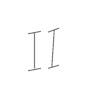
\begin{tikzpicture}\draw[gray] (-.08,.44)--(.08,.47) (0,0)--(0,.45) (-.08,-.03)--(.08,0);\draw[gray] (.22,.02)--(.25,.48) (.17,.46)--(.31,.51) (.17,0)--(.31,.04);\end{tikzpicture}}} $S'=\operatorname{Spec}(\bar A)$, où $A$ est un anneau local noethérien et $\bar A$ son complété; ou encore celui où $S'$ est quasi-fini sur $S$ (i.e. localement isomorphe à un ouvert d'un $S$-schéma fini) et non fini. Dans ces deux cas, \deleted{j'ignore en particulier} le conférencier ignore aussi la réponse à la question suivante: soit $X$ un $S$-schéma tel que $X'=X\times_S S'$ \margin{\figure{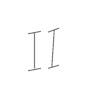
\begin{tikzpicture}\draw[gray] (-.08,.44)--(.08,.47) (0,0)--(0,.45) (-.08,-.03)--(.08,0);\draw[gray] (.22,.02)--(.25,.48) (.17,.46)--(.31,.51) (.17,0)--(.31,.04);\end{tikzpicture}}} soit projectif sur $S'$, est-il vrai que $X$ est projectif sur $S$ ?

2. \uline{Application à la descente de certaines propriétés de morphismes}.- \margin{\figure{\begin{tikzpicture}\draw[gray] (5.8,.2) .. controls (6.2,-.05) and (4.5,-.12) .. (1,-.12) .. controls (-.2,-.14) and (-.3,-.42) .. (0,-.45);\end{tikzpicture}}}

Soit $P$ une \deleted{propriété} \inserted{classe} de morphismes de préschémas. Soit $\alpha:S'\longrightarrow S$ un morphisme de préschémas, \deleted{soient $X,Y$ deux $S$} et soit $f:X\longrightarrow Y$ un morphisme de $S$-préschémas, $f':X'\longrightarrow Y'$ l'image réciproque de $f$ par $\alpha$. On peut se demander alors si la relation \deleted{``$f'$ satisfait $P$''} \inserted{``$f'\in P$''} implique \deleted{``$f$ satisfait} \inserted{``$f\in$} $P$''. \margin{\figure{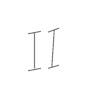
\begin{tikzpicture}\draw[gray] (-.08,.44)--(.08,.47) (0,0)--(0,.45) (-.08,-.03)--(.08,0);\draw[gray] (.22,.02)--(.25,.48) (.17,.46)--(.31,.51) (.17,0)--(.31,.04);\end{tikzpicture}}} Il apparaît que la réponse est affirmative dans beaucoup de cas importants lorsque l'on suppose que $\alpha$ est \uline{fidèlement plat} et \uline{quasi}
\margin{116}

\scanpage{118}
\fbox{\uline{Corollaire} Soit $U$ une partie ouverte de $\operatorname{Spec}(A)$ contenant $\operatorname{Spec}(A_f)$ et les $p_i$,}

\uline{Corollaire 1} Soit $X$ un schéma \uline{affine} sur $A$, et $s$ une section rationnelle de $X/A$, définie dans $\operatorname{Spec}(A_f)$ et aux points $p_i$. Alors $s$ est définie partout.
\figure{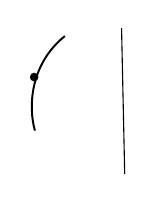
\begin{tikzpicture}[x=1cm,y=1cm]
\draw[line width=.7pt] (.48,1.2) .. controls (.02,.83) and (.02,.27) .. (.1,0);
\fill (.09,.68) circle (.055);
\draw (1.2,1.3)--(1.24,-.55);
\end{tikzpicture}}

Faisant $X=\operatorname{Spec} A[T,T^{-1}]$, on trouve

\uline{Corollaire 2} $A^*=A_f^*\cap\displaystyle\bigcap_i A_{p_i}^*$.

On peut \unsure{énoncer ceci} en disant qu'on a une \inserted{suite exacte de groupes}
\diagram{\begin{tikzcd}[column sep=1.15em,row sep=1.8em]
0 \arrow[r] & A^* \arrow[r] & A_f^* \arrow[r] & \deleted{\unsure{\prod}}\mathbf{Z}^I \arrow[r] & \mathbf{Z}^{\textcircled{\scriptsize I}} \\
&& \figure{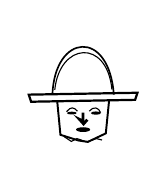
\begin{tikzpicture}[x=.6cm,y=.6cm,baseline=0]
\draw[line width=.6pt] (-.65,.4) .. controls (-.6,1.7) and (.55,1.8) .. (.65,.4);
\draw (-.6,.5) .. controls (-.5,1.5) and (.5,1.6) .. (.61,.51);
\draw[line width=.8pt] (-1.15,.4)--(1.15,.44)--(1.1,.29)--(-1.1,.25)--cycle;
\draw[line width=.7pt] (-.55,.28)--(-.48,-.45)--(-.1,-.57)--(.1,-.6)--(.48,-.42)--(.55,.28);
\draw (-.35,.04) .. controls (-.26,.15) and (-.2,.14) .. (-.12,.05);
\fill (-.24,.01) ellipse (.105 and .03);
\draw (.13,.05) .. controls (.22,.16) and (.33,.13) .. (.37,.02);
\fill (.27,.01) ellipse (.105 and .035);
\draw[line width=1pt] (0,.02)--(0,-.16)--(-.08,-.12)--(.01,-.22)--(.09,-.13);
\fill (0,-.34) ellipse (.15 and .05);
\draw (-.4,-.49)--(-.25,-.59)--(-.13,-.53)--(.07,-.6)--(.28,-.53)--(.4,-.56);
\end{tikzpicture}} && \\
& K^*/A^* \arrow[r] \arrow[d] & K^*/A_f^* \arrow[d] && \\
& \mathbf{Z} \arrow[r] & \mathbf{Z}^I && \\
0 \arrow[r] & A^*\times\mathbf{Z} \arrow[r] & A_f^* \arrow[r] & \mathbf{Z}^I & \\
&& A^*\times\mathbf{Z} \arrow[u] \arrow[r,no head] & \mathbf{Z}^{\deleted{\unsure{I}}} \arrow[u] &
\arrow[from=1-1,to=5-2,no head,out=-50,in=105,looseness=1.3]
\arrow[from=1-1,to=4-2,no head,out=-35,in=170,looseness=1.6]
\arrow[from=1-1,to=1-5,no head,bend left=6]
\arrow[from=1-5,to=5-3,no head,out=-50,in=20,looseness=1.2,line width=1pt]
\arrow[from=1-5,to=3-4,no head,out=-85,in=85,looseness=1.6]
\arrow[from=4-3,to=5-3,no head,out=-145,in=80]
\end{tikzcd}}

\uline{Corollaire 3} Supposons $(f)$ \uline{premier}. Alors \deleted{\unsure{A_f^*}} \deleted{et} $A_f^*\simeq A^*\times\mathbf{Z}$, i.e. \deleted{\unsure{tout}} $t\in A_f^*$ s'écrit de façon unique sous la forme $\varepsilon f^n$, $\varepsilon\in A^*$, $n\in\mathbf{Z}$.
\deleted{\unsure{à diviseur premier}}
\margin{117}

\scanpage{119}
\mspage{19}
d'un faisceau quasi-cohérent d'algèbres commutatives ``équivaut'' à la donnée sur $S'$ d'un tel faisceau, muni d'une donnée de descente relativement à $\alpha:S'\longrightarrow S$. \margin{\figure{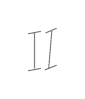
\begin{tikzpicture}\draw[gray] (-.08,.44)--(.08,.47) (0,0)--(0,.45) (-.08,-.03)--(.08,0);\draw[gray] (.18,0)--(.22,.48) (.14,.45)--(.28,.51) (.13,-.02)--(.28,.04);\end{tikzpicture}}} \deleted{Cela} Compte tenu de la correspondance fonctorielle entre de tels faisceaux quasi-cohérents sur $S$, et \inserted{des} préschémas \margin{\figure{\begin{tikzpicture}\draw[gray] (0,0)--(.05,.5);\draw[gray] (.02,.4)--(.2,.45);\end{tikzpicture}}} affines au-dessus de $S$, on obtient la deuxième assertion du théorème suivant:

\uline{Théorème} 2.-Soit $\alpha:S'\longrightarrow S$ \margin{\figure{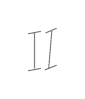
\begin{tikzpicture}\draw[gray] (-.08,.44)--(.08,.47) (0,0)--(0,.45) (-.08,-.03)--(.08,0);\draw[gray] (.18,0)--(.22,.48) (.14,.45)--(.28,.51) (.13,-.02)--(.28,.04);\end{tikzpicture}}} comme dans le théorème 1. Alors $\alpha$ est un \uline{morphisme de descente} (pas strict en général) (\deleted{Par A}, déf\deleted{.}\inserted{\unsure{inition}} 2.4.), et c'est un \uline{morphisme de descente strict} pour la catégorie fibrée des schémas, affines au-dessus de préschémas, (\deleted{Par A}, déf\deleted{.}\inserted{\unsure{inition}} 1.7\deleted{.}).

La première assertion du théorème \unsure{ssgnifie|signifie} ceci: \deleted{S}\inserted{s}oient $X,Y$ deux préschémas \margin{\figure{\begin{tikzpicture}\draw[gray] (0,0)--(.05,.5);\draw[gray] (.02,.4)--(.2,.45);\end{tikzpicture}}} au-dessus de $S$, \margin{\figure{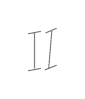
\begin{tikzpicture}\draw[gray] (-.08,.44)--(.08,.47) (0,0)--(0,.45) (-.08,-.03)--(.08,0);\draw[gray] (.18,0)--(.22,.48) (.14,.45)--(.28,.51) (.13,-.02)--(.28,.04);\end{tikzpicture}}} $X',Y'$ leurs images inverses sur $S'$ et $X'',Y''$ leurs images inverses sur $S''\inserted{=S'\times_S S'}$, alors le diagramme suivant d'applications naturelles
\diagram{\begin{tikzcd}
\operatorname{Hom}_S(X,Y) \arrow[r,"\alpha^*"] & \operatorname{Hom}_{S'}(X',Y') \arrow[r,shift left=.7ex,"p_1^*"] \arrow[r,shift right=.7ex,"p_2^*"'] & \operatorname{Hom}_{S''}(X'',Y'')
\end{tikzcd}}
est \uline{exact}, i.e. \margin{\figure{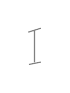
\begin{tikzpicture}\draw[gray] (-.08,.38)--(.08,.43) (0,0)--(0,.4) (-.07,-.03)--(.08,0);\end{tikzpicture}}} \deleted{le premier homomorphisme} \inserted{$\alpha^*$} est une bijection de $\operatorname{Hom}_S(X,Y)$ sur la partie de $\operatorname{Hom}_{S'}(X',Y')$ formé des homomorphismes qui sont compatibles avec les données de descente canoniques sur $X',Y'$ (i.e. \margin{\figure{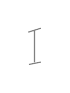
\begin{tikzpicture}\draw[gray] (-.08,.38)--(.08,.43) (0,0)--(0,.4) (-.07,-.03)--(.08,0);\end{tikzpicture}}} dont les images inverses par les deux projections de $S''$ sur $S'$ sont égales). Cela résulte facilement du théorème 1\deleted{.}\inserted{, corollaire 1,} lorsqu'on se borne à $Y$ affine sur $S$; dans le cas général, il faut conjuguer le théorème 1\deleted{\unsure{a}} avec le résultat suivant; \deleted{dont nous ne donnerons pas la démonstration ici}

\margin{\figure{\begin{tikzpicture}\draw[gray] (0,0)--(.45,0)--(.42,.48)--(.65,.52);\draw[gray] (.56,-.08)--(1.2,-.08);\end{tikzpicture}}} \uline{Lemme} 1.2.- Soit $\alpha:S'\longrightarrow S$ \margin{\figure{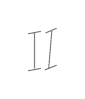
\begin{tikzpicture}\draw[gray] (-.08,.44)--(.08,.47) (0,0)--(0,.45) (-.08,-.03)--(.08,0);\draw[gray] (.18,0)--(.22,.48) (.14,.45)--(.28,.51) (.13,-.02)--(.28,.04);\end{tikzpicture}}} un morphisme fidèlement plat et quasi-compact. Alors $S$ s'identifie à un \uline{espace topologique quotient de} $S'$, i.e. toute partie $U$ de $S$ telle que $\alpha^{-1}(U)$ soit ouverte, est ouverte.

Pour compléter le théorème 2, il faut donner des critères d'effectivité pour une donnée de descente sur un $S'$-préschéma \margin{\figure{\begin{tikzpicture}\draw[gray] (0,0)--(.05,.5);\draw[gray] (.02,.4)--(.2,.45);\end{tikzpicture}}} $X'$ (dans le cas où $X'$ n'est pas supposé affine\deleted{\unsure{s}} sur $S'$). Remarquons d'abord qu'\uline{une telle donnée de descente n'est pas nécessairement effective}, même si $S$ est le spectre d'un corps \inserted{$k$} \margin{\textcircled{$k$}} \margin{\figure{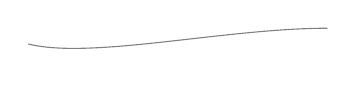
\begin{tikzpicture}\draw[gray] (0,.1) .. controls (.8,-.1) and (2.5,.3) .. (3.8,.3);\end{tikzpicture}}}, $S'$ le spectre d'une extension quadratique \inserted{$k'$} de ce dernier, et $S'$ \deleted{le} un schéma algébrique simple et propre de dimension \deleted{\unsure{2}}\inserted{\unsure{3}} sur $S'$ (comme on peut voir, d'après SERRE, en utilisant la surface non projective de NAGATA). \deleted{On constate} \uline{Pour qu'une donnée de descente sur} $X'/S'$ \uline{relativement à} $\alpha:S'\longrightarrow S$ \margin{\figure{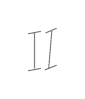
\begin{tikzpicture}\draw[gray] (-.08,.44)--(.08,.47) (0,0)--(0,.45) (-.08,-.03)--(.08,0);\draw[gray] (.18,0)--(.22,.48) (.14,.45)--(.28,.51) (.13,-.02)--(.28,.04);\end{tikzpicture}}} (\uline{fidèlement plat et quasi-compact}) \uline{soit effective}, \uline{il faut et il suffit que} $X'$ \uline{soit réunion}
\margin{118}

\scanpage{120}
\uline{Proposition} $X$ préschéma loc. noethérien \figure{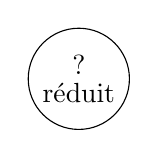
\begin{tikzpicture}\node[draw,circle,inner sep=2pt]{\shortstack{?\\\uline{réduit}}};\end{tikzpicture}}.
\margin{[il suffit $X$ réduit aux pts de $Y$] Car la \unsure{condition} est locale}

$f\in\Gamma(X,\underline{\mathcal O}_X)$, $f$ non diviseur de 0; $Y=\deleted{\unsure{X_f}}V(f)$.

(i) $\underline{\mathcal O}_X/f\underline{\mathcal O}_X$ réduit

\deleted{(ii)} \inserted{($\alpha$) On suppose} les $\underline{\mathcal O}_x$ sont des ``bons'' anneaux, i.e. leurs \unsure{quotients} intègres satisfont i) Condition de finitude ii) Condition des chaînes stricte

Soient $Y_i$ les composantes irréductibles de $Y$.

Soit $Z$ \uline{affine} sur $X$, et $g\deleted{\unsure{\xi}}$ une section rationnelle de $Z$ sur $X$, telle que

(i) $g$ définie dans $X_f$ (ii) $g$ définie en les pts génériques $y_i$ des $Y_i$.

\uline{Alors $g$ est définie partout}
\margin{contre-exemple si $Z$ n'est pas affine ?? $X$ \uline{réduit} est-il essentiel ??}

On est \unsure{ramené au cas où} $X=\operatorname{Spec}(A)$, $A$ local, et où $Z=X[T]$, i.e. $g\in K$ corps des fractions de $A$.

\uline{Lemme 1} Soit $Y$ une partie fermée de $X$ loc. noeth. réduit satisfaisant ($\alpha$), \deleted{$Z$ affine sur $X$} $g$ une \deleted{section} fonction rationnelle de $X$, définie dans $X-Y$ et les points génériques des
\margin{119}

\scanpage{121}
composantes irréductibles de $Z$ qui sont de codim 1 dans $X$. Alors $g$ est \uline{entier} sur $\underline{\mathcal O}_X$.

\uline{Lemme 2} Soit \deleted{$X$ \unsure{comme dessus}, $f$} \deleted{$X,f$ \unsure{comme}} $X$ \deleted{loc} préschéma \deleted{\unsure{f}} réduit, $f$ section de $\underline{\mathcal O}_X$ non diviseur de 0, \inserted{et \deleted{\unsure{tel}} telle que $\underline{\mathcal O}_X/f$ réduit}, $g$ une section de $\underline{\mathcal O}_X$ sur $X_f$, entière sur $\underline{\mathcal O}_X$ en tant que \deleted{section} pseudo-\deleted{sect.}fonction rat. sur $X$. Alors $g$ est partout définie.

\figure{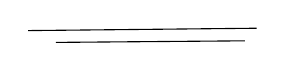
\begin{tikzpicture}[x=1cm,y=1cm]
\draw (0,.15)--(2.9,.18);\draw (.35,0)--(2.75,.02);
\end{tikzpicture}}

\uline{Corollaire 1} Dans les conditions de la proposition, soit $g$ une fonction rationnelle sur $X$. Pour que $g$ soit une section de $\underline{\mathcal O}_X^*$, il f. et s. que $g|X_f$ le soit, et que \deleted{$g$} les $g_{y_i}\in\underline{\mathcal O}_{\unsure{y_i}}^*$. \deleted{\unsure{pour}}
\margin{$\longrightarrow$}

\uline{Corollaire 2} Diagramme exact
\diagram{\begin{tikzcd}
\Gamma(X_f,\underline{\mathcal O}_{X_f}^*) \arrow[r] & \mathbf{Z}^I \\
\Gamma(X,\underline{\mathcal O}_X^*)\times\mathbf{Z} \arrow[u] \arrow[r] & \mathbf{Z} \arrow[u]
\end{tikzcd}}
\margin{120}

\scanpage{122}
\uline{Corollaire 3} Dans les conditions de la proposition, \deleted{considérons le groupe des $D(X)$ des diviseurs loc. principaux} \inserted{Soit $D$ un diviseur loc.} principal sur $X$, \deleted{\unsure{supposons les}} \inserted{soit $n_i$ l'entier déf par $D\cap\underline{\mathcal O}_{y_i}=\unsure{\sigma}(f_{y_i})^{n_i}$ i.e. le coefficient de $Y_i$ dans $D$.} \inserted{Supposons les} conditions suivantes satisfaites
\[
\text{(i)}\quad D\cap X_f=0
\]
(ii) \deleted{$D\cap\underline{\mathcal O}_{y_i}=\unsure{\sigma}(f_i)$} Tous les $n_i$ égaux \inserted{à un \unsure{même} $n$}

Alors $D=n\deleted{(f)}.\operatorname{div}(f)$

\uline{Corollaire 5} (\uline{Non démontré}) \inserted{Dans les conditions de} \deleted{\uline{Prop 4}} Prop, supposons \inserted{(ii) Pour tout $X_\alpha$, $Y\cap X_\alpha$ est irréd. (iii)} $Y$ connexe par la ``relation \deleted{d'équivalence} \inserted{d'incidence}'' suivante: $Y_i$ et $Y_j$ sont \uline{incidents} s'il existe une composante irréductible \inserted{$Z_{ij}\unsure{\subset}Y_i\cap Y_j$} \inserted{\unsure{contenant un|contenue dans un} $Z_{ij}$ de $\unsure{Y_i|X_i}\cap\unsure{Y_j|X_j}$} \deleted{\unsure{qui rencontre} $X_f$. \unsure{telle que la partie}}

Alors \deleted{tout} diviseur \deleted{\unsure{sur}} $D$ sur $X$ tel que $D\cap X_{\unsure{f|g}}=0$ est de la forme $n\operatorname{div}(f)$.

\margin{\uline{N.B} les hypothèses \unsure{faites} impliquent certainement que \unsure{l'on a une correspondance} \uline{biunivoque} \unsure{des composantes de} $X$ \unsure{aux} $Y_i$.
\diagram{\begin{tikzcd}X_\alpha \arrow[r,mapsto] & X_\alpha\cap Y\end{tikzcd}}
\unsure{1°)} $X_\alpha\cap Y$ est un $Y_i$;
\unsure{2°)} $X_\alpha\cap Y=X_\beta\cap Y\Rightarrow\alpha=\beta$
}

\inserted{Cas particulier. Dans les conditions de la Prop}
\uline{Cor \unsure{4|5}} Supposons \deleted{$X$ \unsure{irréd.}} $Y$ irréductible (donc $X$ \unsure{irréd.}
\deleted{Alors} tout $D$ tel que $D\cap X_f=0$, Alors $D=n\operatorname{div}(f)$
\margin{121}

\scanpage{123}
Il suffit en vertu du cor. 3 de vérifier que \deleted{$n_i=n_j$} les $n_i$ sont égaux, donc il suffit de le vérifier \inserted{$n_i=n_j$} pour \deleted{\unsure{tous les}} $Y_i,Y_j$ ``incidents''. \inserted{en prenant $Y_i=Y\cap X_i$, $Y_j=Y\cap X_j$} \deleted{Pour}

Soit $X_{ij}$ une composante irréductible de \deleted{\unsure{ceci}, soit $z$ le pt générique de} $X_i\cap X_j$ \deleted{contenant} $Z_{ij}$ et rencontrant $X_f$. \deleted{$(Z_{ij})$} on peut supposer $X=\operatorname{Spec}A_{\unsure{z}}$; \deleted{$\unsure{A}$} \deleted{donc}\inserted{avec} $D$ \deleted{\unsure{est}} de la forme $\operatorname{div}t$, où $t\in\mathbf R(A)$. Comme $D\cap X_f=0$, on a $t\in A_f^*$,

\figure{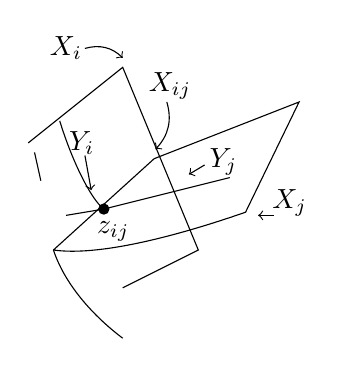
\begin{tikzpicture}[x=0.8cm,y=0.8cm]
\draw (-2,0.8)--(-0.5,2.0)--(0.7,-0.9)--(-0.5,-1.5);
\draw (-1.8,0.2)--(-1.9,0.65);
\draw (-1.6,-0.9) .. controls (-1.4,-1.5) and (-0.9,-2) .. (-0.5,-2.3);
\draw (-1.6,-0.9)--(0,0.55)--(2.3,1.45)--(1.45,-0.3) .. controls (0.3,-0.7) and (-0.9,-1.0) .. (-1.6,-0.9);
\draw (-1.4,-0.35)--(-0.8,-0.25)--(1.2,0.25);
\draw (-1.5,1.15) .. controls (-1.3,0.5) and (-1,-0.1) .. (-0.8,-0.25);
\fill (-0.8,-0.25) circle (0.09);
\node at (-0.65,-0.6) {$\unsure{z_{ij}}$};
\node at (-1.4,2.3) {$X_i$}; \draw[->] (-1.1,2.3) to[bend left] (-0.5,2.15);
\node at (0.25,1.7) {$X_{ij}$}; \draw[->] (0.2,1.45) to[bend left] (0.02,0.7);
\node at (-1.15,0.8) {$Y_i$}; \draw[->] (-1.1,0.6)--(-1,0.05);
\node at (1.1,0.5) {$Y_j$}; \draw[->] (0.8,0.45)--(0.55,0.3);
\node at (2.15,-0.15) {$X_j$}; \draw[->] (1.9,-0.35)--(1.65,-0.35);
\end{tikzpicture}}

\deleted{donc $t=x/f^m$, \inserted{$x\in A$}, Soit $A_i=(X_i)$, $f\mapsto f_i$. En se restreignant à $X_i$, on obt que
\[
t_i=\varepsilon_i f_i^{n_i},\qquad \varepsilon_i\in A_i^*,\quad \deleted{$\unsure{f_i\in K_i}$}\quad n_i\text{ un entier}.
\]
De plus, Comme $Z_{ij}\cap X_f\ne\varnothing$, $t_i|Z_{ij}$ et $t_j|Z_{ij}$}

Soit $t_i=t|X_i$, \inserted{$f_i=f|X_i$, \unsure{cor. 3}} on a
\[
t_i=\varepsilon_i f_i^{n_i}\qquad (\varepsilon_i\in A_i^*,\ n_i\in\mathbf Z).
\]
\figure{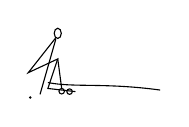
\begin{tikzpicture}[x=0.5cm,y=0.5cm]
\draw (0.2,1.6) ellipse (0.09 and 0.13);
\draw (0.16,1.5)--(-0.55,0.6)--(0.2,0.95)--(-0.05,0.2)--(0.65,0.12);
\draw (0.15,1.45)--(-0.25,0.05);\draw (0.2,0.95)--(0.3,0.2);
\draw (-0.05,0.35) .. controls (0.6,0.22) and (1.4,0.35) .. (2.8,0.16);
\draw (0.3,0.13) circle (0.07);\draw (0.5,0.12) circle (0.07);
\fill (-0.5,-0.03) circle (0.035);
\end{tikzpicture}}

\margin{\unsure{faux ici} ?\quad \fbox{\parbox{0.26\linewidth}{Attention, on ne sait pas si $X_i\times_XY=V(f_i)$ est \uuline{réduit}.}} ?}

\deleted{$Z_{ij}\in X_{ij}$}, $t_i|X_{ij}$ et $t_j|X_{ij}$ existent, et sont égaux, soit $\unsure{t'_{ij}}=\unsure{t'_{ji}}$ \unsure{on a} $=$ \uuline{\unsure{d'où}}.

\unsure{Les sections} \deleted{$t_{ij}=\varepsilon_{ij}f_i$} $f_{ij}=f|\unsure{X_{ij}|Z_{ij}}$, \inserted{$\varepsilon_{ij}=\varepsilon_i|Z_{ij}$, $\varepsilon_{ji}=\varepsilon_j|Z_{ij}$} sont des unités sur $Z_{ij}$.
\margin{122}

\scanpage{124}
On aura évidemment
\[
t_{ij}=\varepsilon_{ij}f_{ij}^{n_i}=\varepsilon_{ji}f_{ji}^{n_j}
\]
\inserted{$\unsure{\varepsilon''_{ij}}f^{n_i}=\varepsilon_{ji}f^{n_j}$}

\deleted{Supp Je dis que} \deleted{\unsure{Supp}} Je dis que $n_i=n_j$. Supposons en effet $n_i>n_j$, on aurait \deleted{$(\varepsilon_{ij}/\varepsilon_{ji})f_{ij}^{n_i-n_j}=1$,} \deleted{et comme}
\[
f_{ij}^{(n_i-n_j)}=\varepsilon_{ji}/\varepsilon_{ij}
\]
donc $f_{ij}$ serait une unité, ce qui \deleted{n'est pas le cas} est absurde puisque $f_{ij}$ s'annule sur $Z_{ij}\subset X_{ij}$.

\margin{\figure{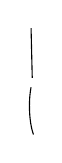
\begin{tikzpicture}[x=0.3cm,y=0.3cm]\draw (0,4.5)--(0.05,2.4);\draw (0,2.0) .. controls (-0.12,1.4) and (-0.08,0.5) .. (0.1,0);\end{tikzpicture}}}
\uline{Théorème}. Soit $f:X\text{---}Y$ un morphisme propre \inserted{et} \uline{séparable}, \inserted{$Y$ loc. noeth. On suppose que $X/Y$ \unsure{0-coh. universellement} \unsure{pour} tt $Y'\leftarrow Y$} \deleted{On suppose que} $n(y)$ le nb des composantes irréductibles \uline{absolues} de $f^{-1}(y)$, et supposons $n(y)$ loc. constant. Soit $\underline L$ un faisceau inversible sur $X$. \deleted{Alors} \inserted{\unsure{On a (i)|On a}} Il existe un plus \unsure{grand} sous-préschéma \deleted{\unsure{fermé}} fermé $Y'$ de $Y$ tel que $\underline L\otimes_Y Y'$ soit isomorphe au faisceau trivial sur $Y$, \unsure{ce est} \deleted{\unsure{appelé}} $S(L/X/Y)$.

(ii) On a.
\[
S(\unsure{L_1^a},X_1,Y_1)\simeq S(L/X/Y)\times_Y Y_1
\]
\margin{123}

\scanpage{125}
Th d'existence

relatifs
\margin{124}

\scanpage{126}
\margin{$p:X'\text{---}X$ un $S$-mph. (On pose $X''=X'\times_X X'$, $X'''=X'\times_X X'\times_X X'$, et on désigne par $f'',f'''$ leurs morphismes \unsure{structuraux}.)}

\margin{\figure{\begin{tikzpicture}[x=0.2cm,y=0.2cm]\draw (-0.8,10)--(-1,9.2);\draw (-0.45,10.2)--(-0.6,9.2);\draw (0,9.8)--(0.12,8.4);\draw (0.15,6.8)--(0.4,0.8);\draw (0.65,0.2)--(0.7,-0.8);\end{tikzpicture}}}
\uline{Proposition}. Soient $f:X\longrightarrow S$ et $f':X'\longrightarrow S$ des morphismes. On suppose $f=(X\xrightarrow{f_1}\Sigma\xrightarrow{f_2}S)$, avec $f_2$ fini \deleted{et $f_1(\mathcal O_X)\simeq\mathcal O_\Sigma$} et de même $f'=(X'\xrightarrow{f'_1}\Sigma'\xrightarrow{f'_2}S)$. On suppose donnée une section $g$ de $X$ sur $\Sigma$, une section $g'$ de $X'$ sur $\Sigma'$, et on désigne par $Z$ le sous-préschéma (fermé) $g(\Sigma)$ de $X$, par $Z',Z''$ ses images \inserted{\unsure{les images}} inverses dans $X',X''$ \inserted{et $Z'\simeq Z\times_\Sigma\Sigma'$} \deleted{et on suppose (i) $g'(\Sigma')\subset Z'$. On suppose de plus $X''=X'\times_X X'$, $X'''=X'\times_X X'\times_X X'$, et on désigne par}

(i) \deleted{$\unsure{X,X'}$} $f_1$, \deleted{$\unsure{\Sigma}$}, $f'_1$, \deleted{$\unsure{\Sigma'}$}, \deleted{$[\unsure{f_2,f'_2}]$}\inserted{$f'',f'''$ et $\Sigma'\text{---}S$, $\Sigma''\longrightarrow S$}, $Z'\longrightarrow\Sigma$ sont plats. \deleted{[\unsure{ainsi que} $f,f',Z'\text{---}\Sigma,Z''\text{---}S$]} $f_1$ et $p$ propres.

(ii) $f_{1*}(\mathcal O_X)\simeq\mathcal O_\Sigma$ et $f'_{1*}(\mathcal O_{X'})\simeq\mathcal O_{\Sigma'}$ \uline{universellement} \deleted{par rapport à $S$}.

(iii) $Z'\longrightarrow Z$ est un morphisme de descente $S$-universel pour les Modules inversibles.

(iv) $p:X'\text{---}X$ est un morphisme de descente \uline{effective} $S$-universel pour les Modules inversibles.

(v) \deleted{$\unsure{g'}$} $g':\Sigma'\longrightarrow X'$ est \unsure{majoré} par $Z'$.

Sous ces conditions, $\underline{\operatorname{Pic}}_{X/S}\longrightarrow \deleted{\prod_{\Sigma'/S}}\underline{\operatorname{Pic}}_{X'/\Sigma'}$ est représentable par des morphismes \uline{affines}.
\inserted{$\underline{\operatorname{Pic}}_{X/S}=\prod_{\Sigma/S}\underline{\operatorname{Pic}}_{X/\Sigma}$}

\uline{Cor}. Si $\underline{\operatorname{Pic}}_{X'/\Sigma'}$ est \deleted{représentable}\inserted{\unsure{exst}}, il en est de même de $\underline{\operatorname{Pic}}_{X/S}$, et $\underline{\operatorname{Pic}}_{X/\Sigma}\longrightarrow\underline{\operatorname{Pic}}_{X'/\Sigma'}$ est un morphisme affine.
\margin{125}

\scanpage{127}
Comme $f_1$ est propre et $\mathcal O_\Sigma\simeq f_{1*}(\mathcal O_X)$ univ\textsuperscript{t}, il s'ensuit \deleted{\unsure{que}} que $\underline{\operatorname{Pic}}_{X/S}(T)$ s'interprète par les $\underline L$ inversibles sur $X_T$ $g_T$-rigidifiés. \unsure{Analogue} pour $\underline{\operatorname{Pic}}_{X'/S'}(T)$. Toutes les hyp. étant stables par extension de la base, on est ramené à ceci: \uline{\unsure{fix}} $\underline L'$ sur $X'$ \uline{avec une $g'$-rigidification $\psi'$} \deleted{\unsure{Reprendre}}. \uline{Prouver que le foncteur} $T\rightsquigarrow$ ens des $\underline L$ $g$-rigidifiés sur $X_T$, tels que $p_T^*(\underline L)\simeq L'_T$ \uline{pour les $g$-rigidif\textsuperscript{ns}}, \uline{est représentable par un schéma affine sur $S$}.

\margin{(i) $f_1,f'_1$ plats $\Sigma\text{---}S$, $\Sigma'\longrightarrow S'$ finis (ii)}
\margin{\fbox{\parbox{0.28\linewidth}{L'hom fonctoriel $\underline{\operatorname{Pic}}_{X/S}\longrightarrow\underline{\operatorname{Pic}}_{X'/S'}$ s'interprète alors de façon simple grâce au fait que $g':\Sigma'\longrightarrow X'$ est majoré par $Z'$ (v)}}}
\margin{\figure{\begin{tikzpicture}[x=0.3cm,y=0.3cm]\draw[->] (3,1.4) .. controls (3.3,0.8) and (0.3,1.1) .. (0,0);\end{tikzpicture}}}

\margin{(iii) (iv)}
Or la donnée de $\underline L$ \uline{équivaut à}:

1°) Un isom $q_{1T}^*(\underline L'_T)\xrightarrow[\sim]{\varphi}q_{2T}^*(\underline L'_T)$
\inserted{$\text{``}\ q_1^*(\underline L')_T\qquad \text{``}\ q_2^*(\underline L')_T$}

2°) Un isom $\underline{\mathcal O}_{Z'}\xrightarrow{\psi}\deleted{\unsure{q_1^*}}i'^*(L'_T)$
\inserted{$\text{``}\ i'^*(\underline L')_T$}

satisfaisant les conditions suivantes
\[
\left\{\begin{aligned}
\text{a) Transitivité}\quad &r_{2T}^*(\varphi)r_{1T}^*(\varphi)=r_{3T}^*(\varphi),\\
\text{b)}\quad &\bar q_{2T}^*(\psi)=i_T''{}^*(\varphi)\bar q_{1T}^*(\psi)\\
\text{c)}\quad &\deleted{\text{Condition de}}\\
&\bar g'_T{}^*(\psi)=\psi'_T
\end{aligned}\right.
\]
\diagram{\begin{tikzcd}[column sep=large,row sep=large]
X & X'\arrow[l,"p"'] & X''\arrow[l,"q_1",shift left=1.1ex,no head]\arrow[l,"q_2"',shift right=1.1ex] & X'''\arrow[l,"{r_1,r_2,r_3}",shift left=1.8ex]\arrow[l]\arrow[l,shift right=1.8ex]\arrow[ll,bend right=65,"{s_1,s_2,s_3}"']\arrow[ll,bend right=50]\arrow[ll,bend right=35]\\
Z\arrow[u,"i"] & Z'\arrow[u,"i'"]\arrow[l,"\bar p"'] & Z''\arrow[u,"i''"]\arrow[l,"\bar q_1",shift left=1.1ex]\arrow[l,"\bar q_2"',shift right=1.1ex] & \\
\Sigma\arrow[u,"\unsure{i}"] & \Sigma'\arrow[u,"\bar g'",very thick] & &
\arrow[phantom,from=1-3,to=1-3,"\ast"{above,yshift=1.7ex}]
\arrow[phantom,from=3-2,to=2-2,"\deleted{\unsure{g'}}"{left}]
\arrow[phantom,from=3-2,to=2-2,"\ast"{above right}]
\end{tikzcd}}

\deleted{On a}
\margin{126}

\scanpage{128}
Or les données 1° et 2° s'expriment par des $S$-morphismes de $T$ ds des $S$-préschémas \deleted{affines} $K,L$ sur $S$ affines sur $S$. Les homomorphismes de $s_1^*(\underline L')_T$ dans $s_2^*(\underline L')_T$, ou de \deleted{$\unsure{(q_1i'')^*(\underline L')_T}$} $\mathcal O_T$ dans $(q_2i'')(\underline L')_T$, \inserted{ou de $\mathcal O_{\unsure{Z''|Z'}}$ dans $(i'\bar q_1)^*(\underline L')$,} \deleted{s'expriment également par des homomorphismes ds des \unsure{puis} $S$-schémas $M,N$ affines sur $S$, et de \unsure{la section} de $(i'\bar g')^*(\underline L')$ sur $\Sigma'$} s'expriment par des $S$-morphismes ds des $S$-préschémas $M,N,P$ \deleted{\unsure{et}} affines sur $S$, donc séparés sur $S$.

\margin{$f''$ et $Z'\longrightarrow S$ plats (i)}
\margin{$f'''$ et $Z''\text{---}S$ plats \inserted{et $\Sigma'\text{---}S$} (i)}

Les conditions écrites a) b) c) s'expriment par le fait que deux \inserted{couples} morphismes
\diagram{\begin{tikzcd}[column sep=small]
K\arrow[r,shift left=0.6ex]\arrow[r,shift right=0.6ex] & M, & L\arrow[r,shift left=0.6ex]\arrow[r,shift right=0.6ex] & N, & L\arrow[r,shift left=0.6ex]\arrow[r,shift right=0.6ex] & P
\end{tikzcd}}
s'égalisent.

Donc si \deleted{$R,S$} $U,V$ sont les noyaux des doubles flèches $K\rightrightarrows M$ et $L\rightrightarrows N\times P$ resp. [qui sont fermés ds $K,L$, donc affines sur $S$] le foncteur envisagé est représenté par $U\times V$, cqfd.
\margin{127}

\scanpage{129}
\deleted{Or les données 1°, 2° correspondent resp. à des \deleted{sections}\inserted{\unsure{points}} de préschémas affines $\unsure{K_T},\unsure{L_T}$ sur $S$, \inserted{[puisque $Z',X''$ \inserted{propres et} plats sur $S$]} donc 1° et 2° à une section de $K\times L$ sur $S$. \deleted{\unsure{et}} D'autre part, les isom de $(L_1''')_T$ sur $(L_3''')_T$ correspondent aux \deleted{des} sections \deleted{de $R$} un $M_T$ affine, \deleted{sur $S$} et ceux de $\mathcal O_{Z''_T}$ sur $i''_T{}^*(L_1'')$ aux sections d'un $N_T$ affine \deleted{\unsure{sur}} \inserted{[car $X''',Z''$ propres et plats sur $S$]} Les conditions a) et b) s'expriment donc en \deleted{disant} faisant coïncider des morphismes donnés
\diagram{\begin{tikzcd}[column sep=small]
K\arrow[r,shift left=0.6ex]\arrow[r,shift right=0.6ex]&M,&L\arrow[r,shift left=0.6ex]\arrow[r,shift right=0.6ex]&N
\end{tikzcd}}
de $K\times M\rightrightarrows L\times N$. Donc on trouve un sous-présch. fermé de $K\times M$. Cela achève la démonstration.}

\margin{\figure{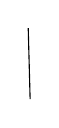
\begin{tikzpicture}[x=0.3cm,y=0.3cm]\draw (0,3)--(0.08,0);\fill (0.055,1.45) circle (0.025);\fill (0.07,0.65) circle (0.025);\end{tikzpicture}}}
\uline{Corollaire}. $X$ séparable et complet sur le corps $k$. \deleted{Supposons les $\underline{\operatorname{Pic}}_{X_i/k}$ existent.}\inserted{\unsure{A}} \deleted{Alors $\underline{\operatorname{Pic}}_{X/k}$ existe.} Soit $X_i$ les composantes \inserted{(réduites)} \deleted{\unsure{des} $X_i$ \unsure{sont irrédu} de $X$}, \deleted{\unsure{sont}} considérons $\underline{\operatorname{Pic}}_{X/k}\text{---}\prod_i\underline{\operatorname{Pic}}_{X_i/k}$, \inserted{cet hom} \deleted{\unsure{trouve} le noyau est affine} \deleted{est affine}. représentable par des morphismes affines. donc si les $\underline{\operatorname{Pic}}_{X_i/k}$ existent, de même $\underline{\operatorname{Pic}}_{X/k}$.
\margin{128}

\scanpage{130}
\mspage{0-ii}
$\Gamma_U(f_\alpha):\Gamma(U,\underline F_\alpha)\longrightarrow\Gamma(U,\underline G_\alpha)$ forment un système projectif d'homomorphismes, les diagrammes
\diagram{\begin{tikzcd}
\Gamma(U,\underline F_\alpha)\arrow[r]\arrow[d]&\Gamma(U,\underline G_\alpha)\arrow[d]\\
\Gamma(V,\underline F_\alpha)\arrow[r]&\Gamma(V,\underline G_\alpha)
\end{tikzcd}}
\figure{\begin{tikzpicture}[x=0.3cm,y=0.3cm]\draw (0,0)--(0.02,0.5)--(-0.12,1.2);\draw (2.2,0)--(2.2,0.7)--(1.7,1.1);\end{tikzpicture}}
étant en outre commutatifs pour $U\supset V$; on en conclut que si $f_U=\varprojlim\Gamma_U(f_\alpha)$, les homomorphismes $f_U$ définissent un homomorphisme de faisceaux $f:\varprojlim\underline F_\alpha\longrightarrow\varprojlim\underline G_\alpha$, que l'on désigne par $\varprojlim f_\alpha$.

On peut donc dire que $\varprojlim$ est un \uline{foncteur} de la catégorie des systèmes projectifs de faisceaux de groupes abéliens sur $X$ dans la catégorie des faisceaux de groupes abéliens sur $X$. Ce foncteur est \uline{exact à gauche}: autrement dit, si \deleted{\unsure{pour chaque} \illegible{3}} $(\underline F'_\alpha)$, $(\underline F_\alpha)$, $(\underline F''_\alpha)$ sont trois systèmes projectifs de faisceaux de groupes abéliens sur $X$, et si pour chaque $\alpha$, on a une suite exacte avec commutativité des diagrammes
\diagram{\begin{tikzcd}
0\arrow[r]&\underline F'_\beta\arrow[r,"f_\beta"]\arrow[d]&\underline F_\beta\arrow[r,"g_\beta"]\arrow[d]&\underline F''_\beta\arrow[d]\\
0\arrow[r]&\underline F'_\alpha\arrow[r,"f_\alpha"]&\underline F_\alpha\arrow[r,"g_\alpha"]&\underline F''_\alpha
\end{tikzcd}}
pour $\alpha\leq\beta$, alors en posant $f=\varprojlim f_\alpha$, $g=\varprojlim g_\alpha$, la suite
\diagram{\begin{tikzcd}
0\arrow[r]&\varprojlim\underline F'_\alpha\arrow[r]&\varprojlim\underline F_\alpha\arrow[r]&\varprojlim\underline F''_\alpha
\end{tikzcd}}
est exacte. Cela résulte aussitôt de ce que le foncteur $\Gamma$ est exact à gauche, et de la propriété correspondante pour le foncteur $\varprojlim$ dans la catégorie des systèmes projectifs de groupes abéliens.

Soit $\varphi$ une application continue de $X$ dans un espace topologique $Y$. Si $(\underline F_\alpha)$ est un système projectif de faisceaux de groupes abéliens sur $X$, on a
\[
\varphi_*(\varprojlim\underline F_\alpha)=\varprojlim\varphi_*(\underline F_\alpha).
\]
En effet, pour tout ouvert $V\subset Y$; on a par définition
\[
\begin{aligned}
\Gamma(V,\varprojlim\varphi_*(\underline F_\alpha))&=\varprojlim\Gamma(V,\varphi_*(\underline F_\alpha))=\varprojlim\Gamma(\varphi^{-1}(V),\underline F_\alpha)\\
&=\Gamma(\varphi^{-1}(V),\varprojlim\underline F_\alpha)=\Gamma(V,\varphi_*(\varprojlim\underline F_\alpha))
\end{aligned}
\]
\margin{129}

\scanpage{131}
Résulte par récurrence \deleted{\unsure{sur}} du

\margin{\figure{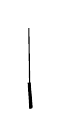
\begin{tikzpicture}[x=0.3cm,y=0.3cm]\draw (0,3.4)--(0.05,0);\draw[line width=1pt] (0.01,1.1)--(0.08,0);\draw (0.05,1.1)--(0.14,0.04);\end{tikzpicture}}}
\uline{Lemme}. $X$ \deleted{séparable}\inserted{\deleted{\unsure{réduit}}\unsure{séparable}} propre sur le corps $k$, et \deleted{soit} $X_1$ et $X_2$ deux parties fermées de $X$, séparables sur $k$, telles que $X=\cup X_1\cup X_2$. Alors $\underline{\operatorname{Pic}}_{X/k}\text{---}\underline{\operatorname{Pic}}_{X_1/k}\times\underline{\operatorname{Pic}}_{X_2/k}$ est représentable par morphismes affines.

\inserted{\deleted{Si $X_1\cap X_2=\varnothing$, \unsure{on a} \unsure{donc}} Supposons $X_1\cap X_2\ne\varnothing$}
Comme les faisceaux en jeu sont compatibles \deleted{\unsure{pour}} aux changements fid plats quasi cpcts, et que \deleted{les} morphismes de cette nature sont des morphismes de descente effective pour les morphismes affines, rien n'est changé en faisant un changement de base $\unsure{\bar k'|k'}/k$, où $k'/k$ est une extension de corps. On peut donc se ramener au cas où $F=X_1\cap X_2$ a un pt rat. sur $k$, i.e. une section $g$ sur $S=\operatorname{Spec}k$), On applique alors le th. avec $X'=X_1\amalg X_2$.

\deleted{\unsure{Dém.}}

\uline{Attention}. Commençons par le corollaire: se ramener au cas où $k$ est alg. clos, et $X$ connexe, ce qui nous ramène dans le \uline{lemme} dans le cas où $X_1$ et $X_2$ sont \uline{connexes} et $X_1\cap X_2$ a un pt rat. /$k$. \unsure{On est ds les conditions du}

\margin{\diagram{\begin{tikzcd}[column sep=small,row sep=large]
\underline{\operatorname{Pic}}_X\arrow[r,"\unsure{\sim}"]\arrow[d,"\text{affine}"'] & \prod_i\underline{\operatorname{Pic}}_{X_i}\\
\underline{\operatorname{Pic}}_{X'}\times\underline{\operatorname{Pic}}_{X''}\arrow[ur,"\text{affine}"'] &
\end{tikzcd}}}
\margin{130}

\scanpage{132}
Par 2 \uline{Etude cohomologique des morphismes \unsure{projectifs}.}

1. \uline{Calculs Explicites de certains groupes de cohomologie}

Soient $X$ un preschema, $\underline L$ un faisceau inversible sur $X$, considerons l'anneau gradue $S=\mathrm I_*(X,\underline L)$ et considerons des $f_i\quad S_{d_i}$ ($1\quad i\quad k$, les $d_i$ des entiers), soit $U_i=X_{f_i}$, $U=\cup U_i$, $\underline U$ le recouvrement \deleted{\unsure{forme}} de $U$ forme par les $U_i$. Si maintenant $F$ est un faisceau quasi-coherent quelconque sur $X$, on posera
\[
\begin{aligned}
F(*)&=\qquad F(\underline L^n\\
H^*(U,F(*))&=\qquad H^*(U,F\quad\underline L^n)\\
H^*(\underline U,F(*))&=\qquad H^*(\underline U,\unsure{R}\quad\underline L^n)
\end{aligned}
\]
Ce sont tous des $S$-modules gradues. Considerons de meme le $S$-module gradue
\[
M=H^0(X,F(*))=\mathrm I(X,F(*))
\]
On aura alors
\[
\mathrm I(U_{i_0i_1\ldots i_p},F(*))=M_{f_{i_0}f_{i_1}\ldots f_{i_p}}=\lim M^{(f_{i_0}f_{i_1}\ldots f_{i_p})^n}
\]
en vertu du Chapitre II, par.1,

en supposant maintenant $X$ noetherien, ou quasi-compact separe); les homomorphismes dans le systeme inductif du dernier membre etant encore la multiplication par $(f_{i_0}f_{i_1}\deleted{\unsure{xxx}}\ldots f_{i_p})^{m-n}$. On en deduit encore, comme au par. precedent:
\[
C^p(\underline U,F(*))=\lim C_n^p(M)
\]
ou $C_n^p(M)$ est forme des fonctions alternees de $p+1$ indices entre $1$ et $k$, a valeurs dans $M$, i.e. pour $p\quad0$ s'identifie a $K^{p+1}(\underline f^n,M)$, les homomorphismes dans ce systeme inductif etant alors les $\underline f^{m-n}$. Par suite on a encore un \deleted{\unsure{homomor}} isomorphisme
\[
C^p(\underline U,F(*))=C^{p+1}\unsure{\}}(\underline f),M)\qquad\text{pour }p\quad0
\]
et ces isomorphismes sont compatibles avec les operateurs differentiels. On fera cependant attention aux questions de degres dans l'isomorphisme precedent; il y a deux degres, celui provenant de $C^*$ et celui provenant de $F(*)$. Dans le deuxieme membre, considere comme limite inductive des $K^{p+1}(\underline f^n,M)$, le \inserted{deuxieme} degre d'une fonction \deleted{\unsure{primitive}} alternee de $p+1$ arguments $i_\alpha$ compris entre $1$ et $k$, a valeurs dans $M_m$, est egal a
\[
m-n(d_{i_1}+d_{i_2}+\ldots+d_{i_p})
\]
Des isomorphismes precedents, on tire la proposition suivante, qui generalise la prop.2 du paragraphe 1:
\margin{131}
